% mn2esample.tex
%
% v2.1 released 22nd May 2002 (G. Hutton)
%
% The mnsample.tex file has been amended to highlight
% the proper use of LaTeX2e code with the class file
% and using natbib cross-referencing. These changes
% do not reflect the original paper by A. V. Raveendran.
%
% Previous versions of this sample document were
% compatible with the LaTeX 2.09 style file mn.sty
% v1.2 released 5th September 1994 (M. Reed)
% v1.1 released 18th July 1994
% v1.0 released 28th January 1994
\pdfoutput=1

\documentclass[useAMS,usenatbib,times,letter,amssymb]{mn2e}
\usepackage{graphicx, float, amsmath,epsfig,times,amssymb,color,verbatim, widetext }
% If your system does not have the AMS fonts version 2.0 installed, then
% remove the useAMS option.
%
% useAMS allows you to obtain upright Greek characters.
% e.g. \umu, \upi etc.  See the section on "Upright Greek characters" in
% this guide for further information.
%
% If you are using AMS 2.0 fonts, bold math letters/symbols are available
% at a larger range of sizes for NFSS release 1 and 2 (using \boldmath or
% preferably \bmath).
%
% The usenatbib command allows the use of Patrick Daly's natbib.sty for
% cross-referencing.
%
% If you wish to typeset the paper in Times font (if you do not have the
% PostScript Type 1 Computer Modern fonts you will need to do this to gets

% smoother fonts in a PDF file) then uncomment the next line
% \usepackage{Times}

%%%%% AUTHORS - PLACE YOUR OWN MACROS HERE %%%%%
\def\be{\begin{equation}}
\def\ee{\end{equation}}
\def\bea{\begin{eqnarray}}
\def\eea{\end{eqnarray}}
\def\lg10{\log_{10}}
\def\T{\theta}
\newcommand{\bm}[1]{\mbox{\boldmath{$#1$}}}   %this is bold italic for MNRAS
%%%%%%%%%%%%%%%%%%%%%%%%%%%%%%%%%%%%%%%%%%%%%%%%

\title[Mass profile reconstruction with magnification]{Cluster Mass Profile Reconstruction with Size- and Flux- Magnification on STAGES data}



\author[C. Duncan et al.]{Christopher A. J. Duncan$^{1}$\thanks{Email: cajd@roe.ac.uk} et al\\% , Catherine Heymans$^{1}$, Alan F. Heavens$^{2}$, Benjamin Joachimi$^{3}$\\
$^{1}$Scottish Universities Physics Alliance, Institute for Astronomy, University of Edinburgh, Royal Observatory, Blackford Hill, Edinburgh, EH9 3HJ, UK\\
$^{2}$Imperial Centre for Inference and Cosmology, Imperial College London, Blackett Laboratory, Prince Consort Road, London, SW7 2AZ, UK.\\
$^{3}$Department of Physics and Astronomy, University College London, Gower Place, London, WC1E 6BT, UK.}

\par

\pdfminorversion=5
\voffset = -0.6in
\begin{document}

\date{Not Yet Accepted}

\pagerange{\pageref{firstpage}--\pageref{lastpage}} \pubyear{2015}

\maketitle

\label{firstpage}

\begin{abstract}
Abstract.
\end{abstract}

\begin{keywords}
Keywords.
\end{keywords}

\section{Introduction}

%%General introduction to clusters, motivation for need to measure mass of clusters - Simet is a good reference
Galaxy clusters comprise the largest known gravitationally bound objects in the Universe which form in the largest peaks of the density field and can give information on the formation of structure and the cosmological model through knowledge of the underlying density field or the large mass end of the mass function. In order to interpret cluster counts in a cosmological scenario, one must have knowledge of the individual masses of the clusters that enter into the sample. Many different observables are commonly used as a proxy for cluster mass, including the use of visible tracers of the underlying matter distribution such cluster member counts (cluster richness) which rely on visible galaxies or X-Ray luminosity and temperature or the Sunyaev-Zeldovich effect which rely on hot gas. In each of these cases, one must make simplifying assumptions on how these tracers follow the underlying dominant dark matter distribution and which must be taken into account when interpreting the measurement as a proxy for the mass of the cluster. For the use of cluster members in the optical this requires knowledge of the galaxy bias, whilst for X-Ray derived masses one must assume hydrostatic equilibrium, whilst recent studies suggest that X-Ray derived masses may be biased low \citep{Simet:2015p2852}. By contrast, gravitational lensing uses measurements of background galaxy size, shape or luminosity to probe the lensing matter distribution, and is insensitive to the nature of the lensing matter itself.

%As photons emitted by distant sources propagate through the Universe, their path of propagation is bent by the presence of intervening matter density contrasts, leading to an alteration in the shape, size, brightness and position of the observed image of the source in a manner which is dependent on the magnitude of the foreground density contrast and the geometry of the lens-source system. The former of these effects is frequently referred to as a shear analysis, and statistical measures of the small distortion in a sample of source ellipticities has been successfully been applied many times to the determination of dark matter profiles on galactic (references) and cluster scales (references), as well as the measurement of cosmological parameters (references). The magnification effect formally labels the (de-)amplification of the source, but more informally various combinations of the latter three effects are frequently collected for various magnification observables: in particular, the alteration in clustering properties of sources around foreground lenses in a flux-limited survey, termed the `magnification bias' or often just `flux magnification', incorporates the fluctuations in the clustering as a result of the change in source position as well as amplification (or de-amplification) of the sources as sources are brought above or below the flux limit of the survey. Similarly, the alteration in flux and size of the object are linked through the application of Liouville's theorem, so that statistical measures of source size may be used as a probe of the lensing medium.

With few exceptions, the use of gravitational lensing measurements as a method of mass reconstruction deal exclusively with the shape distortion of distant sources since the intrinsic dispersion in ellipticity measures is markedly smaller than those for size, magnitude or number density, giving a smaller statistical error for ellipticity analyses using the same number density of sources. As a result of the dominance of the shear statistic in gravitational lensing studies, much time has been invested in developing the tools to accurately use shear measurements. As an example, competitive analyses of the accuracy and precision of weak lensing observable measurement, such as the STEP and GREAT programs, have focussed their attention on testing the ability of particular algorithms in measuring source ellipticity. Whilst many of the techniques considered can also provide an estimate of source size, these have not been the focus of such analyses. Ideally, one would like to utilise the maximum number of independent probes in weak lensing analyses, as a means of reducing the statistical errors on measurements for a given source sample, but also as a means of mitigating systematics in each individual analysis. %For a traditional shear analysis, these include systematics in source shape measurement caused by optical distortions 

There has, however, been a recent increasing trend in investigations into the use of other weak lensing observables. In the recent past, there have been numerous convincing detections of fluctuations in source counts due to lensing by foreground matter, most frequently dubbed `flux magnification' or `magnification bias' through the use of angular correlation functions between radially separated bins \citep{Myers:2003p2024,Scranton:2005p1124,Hildebrandt:2009p845,Morrison:2012p1286}, and around stacked foreground over densities as a means of measuring stacked mass profiles \citep{Ford:2014p2751,Ford:2014p2825,Bauer:2011p2066,Umetsu:2014p2726,Hildebrandt:2011p2755} or determining dust profiles \citep{Menard:2010p1495,Hildebrandt:2013p2756}. Of particular note, the analyses of \citep{Hildebrandt:2011p2755,Hildebrandt:2013p2756} measure the mass profiles for high redshift lenses, using a high redshift background source sample where shape determination would be expected to fail, and thus utilises one of the main strengths of a number-counts magnification analysis.   

Contemporaneously, there have been a series of theoretical investigations into the use of the magnification bias signal to measure cosmological parameters, through the clustering of a photometric sample in \cite{Duncan:2014p2569,Joachimi:2010p855,Waerbeke:2010p7,2010MNRAS.401.2093V} or a part of a joint analysis using a photometric and spectroscopic sample \citep{Gaztanaga:2012p1194,Eriksen:2015p2849}. It is generally found that whilst the magnification bias alone is uncompetitive to shear when an unknown galaxy bias must be simultaneously measured with the data, the combination of clustering and shear can give a significant increase in constraining power over the shear-only signal through degeneracy breaking between the clustering, shear and galaxy-galaxy lensing. Further, \cite{Joachimi:2010p855} found that the addition of existing number density information to a shear analysis on a photometric sample can successfully counteract the loss of information due to the marginalisation over a flexible intrinsic alignment model. As a result, such a combined analysis was adopted as part of the primary science driver in Euclid \citep{Laureijs:2011p2021}, however in \cite{Duncan:2014p2569} it was shown that systematic uncertainties in the magnification bias signal can lead to catastrophic biases in cosmological model parameters.

Similarly, there has been a recent uptake in investigations into the direct use of size and magnitude measurements to infer lensing properties, either through a comparison in statistics of lensed samples to unlensed samples \citep{Heavens:2013p1550,Alsing:2014p2846,Casaponsa:2013p1480}, or through the use of the fundamental plane relation \citep{Huff:2011p1392,Sonnenfeld:2011p1035,Bertin:2006p2063} . In each case, major astrophysical systematics, similar to intrinsic alignments for a shear analysis, may be present through intrinsic size-density correlations \citep{Ciarlariello:2014p2844}, or the correlation between fundamental plane residuals and density \citep{2015arXiv150402662J}.  In \cite{Heavens:2013p1550} it was demonstrated that substantial gains could be made in the combination of a size magnification measurement with a shear analysis, particularly when noise dominated, and noted that the noise-free size measurement can be made to be uncorrelated to the shear measurement, allowing maximum statistical gain from the combination of size and shape, provided that the size is measured as the square-root of a measured source area. In \cite{Alsing:2014p2846} this was taken further, and the authors forecast using a theoretically motivated linear alignment and intrinsic-size-density correlation model that the combination of size and magnitude magnification with shear can give improvements in dark energy parameter space of $\sim 25\to65\%$, whilst quantifying the typical dispersion on the inferred convergence field using an intrinsic size-magnitude distribution measured with CFHTLenS. Similarly, \cite{Rozo:2010p1496} forecast an improvement of $\sim 50\%$ in cluster mass estimates from a joint size- magnification, clustering and shear analysis over shear-only, however \cite{Eifler:2013p2722} found that constraints on a set of cosmological parameters from a non-tomographic COSEBI shear analysis were significantly improved with the addition of projected clustering information, but that the further inclusion of size magnification did not give significant further improvement. In \cite{Casaponsa:2013p1480} it was shown through the use of image simulations that size measurements using LensFit \cite{Miller:2007p2375} could estimate the convergence field in an unbiased way provided the source sample was selected to be above a flux signal--to--noise ratio of $10$, and the galaxies are larger than the point spread function, and suggesting that high resolution space-based imaging is ideal for a size-magnification analysis. 
%Fundamental Plane - systematics - fundamental plane residuals and LSS (Joachimi)
%Direct measure - (Theory and forecasts) Alsing, Heavens, Casaponsa - systematics - ISC (Ciarlariello 2014
%Forecast - Cluster lensing - Rozo and Schmidt
%Measurement - Schmidt.
A recent observational application of the use of the size and magnitude magnification effect is the application in \cite{Schmidt:2012p1106} to stacked group lensing in the COSMOS field. In this paper, authors claim a detection of the magnification effect with a signal--to--noise ratio of $\sim 40\%$ of the shear using a maximum-likelihood estimator based around the assumption of log-normality in the size distribution and Gaussianity in the magnitude distribution. Sizes are measured using quadrupole moments, using the optical-distortion correction of \cite{Rhodes:2000p2068} applied at quadrupole level. It is precisely this signal which is the main aim of this paper, however we instead apply our method of mass estimation using galaxy sizes and magnitudes to individual large clusters of $M=  O(10^{14}) M_{\odot}/h$ on the STAGES field. In Section \ref{sec:TheoryAndMethod} we detail the origin of the weak lensing signal, and detail a Bayesian method for determining cluster model parameters for a given lens from source size, magnitude and ellipticity measurements avoiding some of the simplifying assumptions of previous analyses, and discuss how a joint analysis using all three observables could be combined in a self-consistent way. In Section \ref{sec:STAGESDataset} we describe the STAGES dataset. In Section \ref{sec:ApplicationToMocks}, the method is applied to mock catalogues designed to reflect the main features of the data-set, and conclusions are drawn on the ability to utilise the method to measure cluster model parameters on different mass lenses, and quantify the effect of limitations in the data-set and simplifying assumptions. Finally, in Section \ref{sec:ApplicationToSTAGES} the method is applied to the STAGES dataset, results are presented for the STAGES super-cluster and compared to pre-existing shear measurements. 

\section{Theory and Method}\label{sec:TheoryAndMethod}
\subsection{Weak Lensing Theory}

As photons propagate past a foreground matter density contrast, its path is deflected according to the Jacobian mapping
\be
\mathcal{A} = (1-\kappa) \begin{pmatrix} 1 -g_1 & -g_2 \\ -g_2 & 1+g_1  \end{pmatrix}
\ee
where the Jacobian describes the mapping from the lens to the source plane, in the linear limit. As a result, light emitted from distant sources which is lensed tidally according to the potential of the lensing matter, and observed image of the source is distorted according to the Jacobian above, where the convergence ($\kappa$) and shear ($\gamma$) vary with angular position on the sky and are functions of gravitational potential of the lens and geometry of the lens-source system. The convergence denotes an isotropic stretching of the source image, with a corresponding change in the observed size of the source. Further, as a result of the applicability of Liouville's Theorem, this change in source size corresponds directly to a change in the observed flux of the source. Consequently, the lensed size and flux of a source can be related to its unlensed quantities according to 
\bea
\theta &=& \mu^{\frac{1}{2}}\theta_0 \label{eqn:Lensing_Relations__Size}\\
S &=& \mu S_0 \label{eqn:Lensing_Relations__Flux}\\
m &=& m_0 +2.5\lg10{\mu}, \label{eqn:Lensing_Relations__Magnitude}
\eea
where $\theta$, $S$ and $m$ represent the sources size, flux and magnitude respectively, subscript ``$0$'' denotes intrinsic (or unlensed) quantities, and the local magnification factor $\mu$ is given by the inverse of the Jacobian as
\be
\mu = [\det(\mathcal{A})]^{-1} = [(1-\kappa)^2 - \gamma^2]^{-1}.
\ee
 This parameterisation will be consistently used throughout this paper. The action of the a magnification field is therefore to alter the size and brightness of a lensed source, or locally shift the size-magnitude distribution for the source sample (see Figure \ref{fig:Size_Mag_Lensing_Example}). Equivalently, one may consider the action of the magnification field as a shift in the survey size and flux limits: together with changes in the observed position of the sources, this forms the basis of flux-magnification analyses through clustering statistics (also known as magnification bias), and is not considered here. 

Under the weak lensing assumption ($\kappa, \gamma \ll 1$), the magnification can be simplified to $\mu \sim 1+2\kappa$, allowing for the linearisation of Equations \ref{eqn:Lensing_Relations__Size} to \ref{eqn:Lensing_Relations__Flux} and potentially simplifying the analysis, however, in the method presented here such a simplification is unnecessary, and the relations given above are taken throughout unless otherwise stated. Taken together, this amplification of the magnitude or flux and change in source size are referred to as the `magnification' of the source. One can see that if one has knowledge of the intrinsic size or brightness of an imaged source, one can infer knowledge of the local magnification acting on the source by foreground mass and as a result obtain information on the projected mass along the line of sight. However, in reality, one only has access to the lensed images of distant sources, and as a result one cannot take measurements from a single source without a-priori knowledge of the distribution of intrinsic sizes and magnitudes for a sample of like sources. The measurement can therefore only be made statistically. A common frequentist approach is to construct an estimator for the local magnification factor according to the statistics of the source sample, from which a maximum-likelihood estimate can be sought under certain assumptions on the distribution of the estimate: in this case, the estimator may be constructed from size measurements only as
\be
\hat{\mu} =  \left(\frac{\langle \theta \rangle}{\langle \theta \rangle}_{\rm field}\right)^2
\ee
where the numerator corresponds to the mean size of the source sample, and the numerator corresponds to the mean size over the whole field, assumed to be an unbiased estimator of the mean of the distribution of intrinsic sizes for the sample considered. As similar estimator can be constructed for the flux-magnification effect, however such an estimator will share many similarities with the size-magnification estimator above, and is ignored for now. 

The use of such an estimator requires special care. When the source or field sample is chosen within a given flux of magnitude range, any intrinsic size-luminosity relation must be taken into account to account for the flux-lensing of the sample, and to ensure that the estimator compares mean sizes of equivalent samples: if this is not the case, such an estimator is likely to be biased. The estimator gives an estimate for the average magnification factor for the source sample, and as such its physical interpretation is more difficult when the source sample is chosen over an area where the magnification factor can be expected to vary significantly. Such difficulties can be avoided by choosing the sample in a small patch of sky, or azimuthally averaging the magnification where a spherically symmetric lens mass profile is assumed. Moreover, the estimator is likely to be biased if the assumption that the field mean is not representative of the true unlensed mean of the sample is false. Such a case can arise where the average magnification across the field is not uniform, for example where the field is small and dominated by a large over-density such as a cluster, or an under-density such as a void. To avoid such bias, the field mean should be calculated over as large a volume as possible, or using a blank field where large volumes are not available.

Whilst the use of such an estimator is viable, and has been the subject of a number of papers which aim to set out the framework for such a measurement \citep[e.g.][]{Heavens:2013p1550,Alsing:2014p2846,Casaponsa:2013p1480} each of these biases must be taken into consideration to assure the estimator is unbiased. As such, this paper motivates a deviation from such a formalism, and in the next section I present a Bayesian method of constraining parameters for the mass profile of the lens where the intrinsic size-magnitude distribution is fully modelled. In such a formalism, any intrinsic correlation between the size and magnitude measures is encompassed in the field size-magnitude distribution, negating the need for any correction due to this effect. Further, the method can be applied to produce lens mass profile constraints on a single-galaxy level, simplifying the interpretation of the measurements for a chosen sample of sources.

\begin{figure*}
\centering
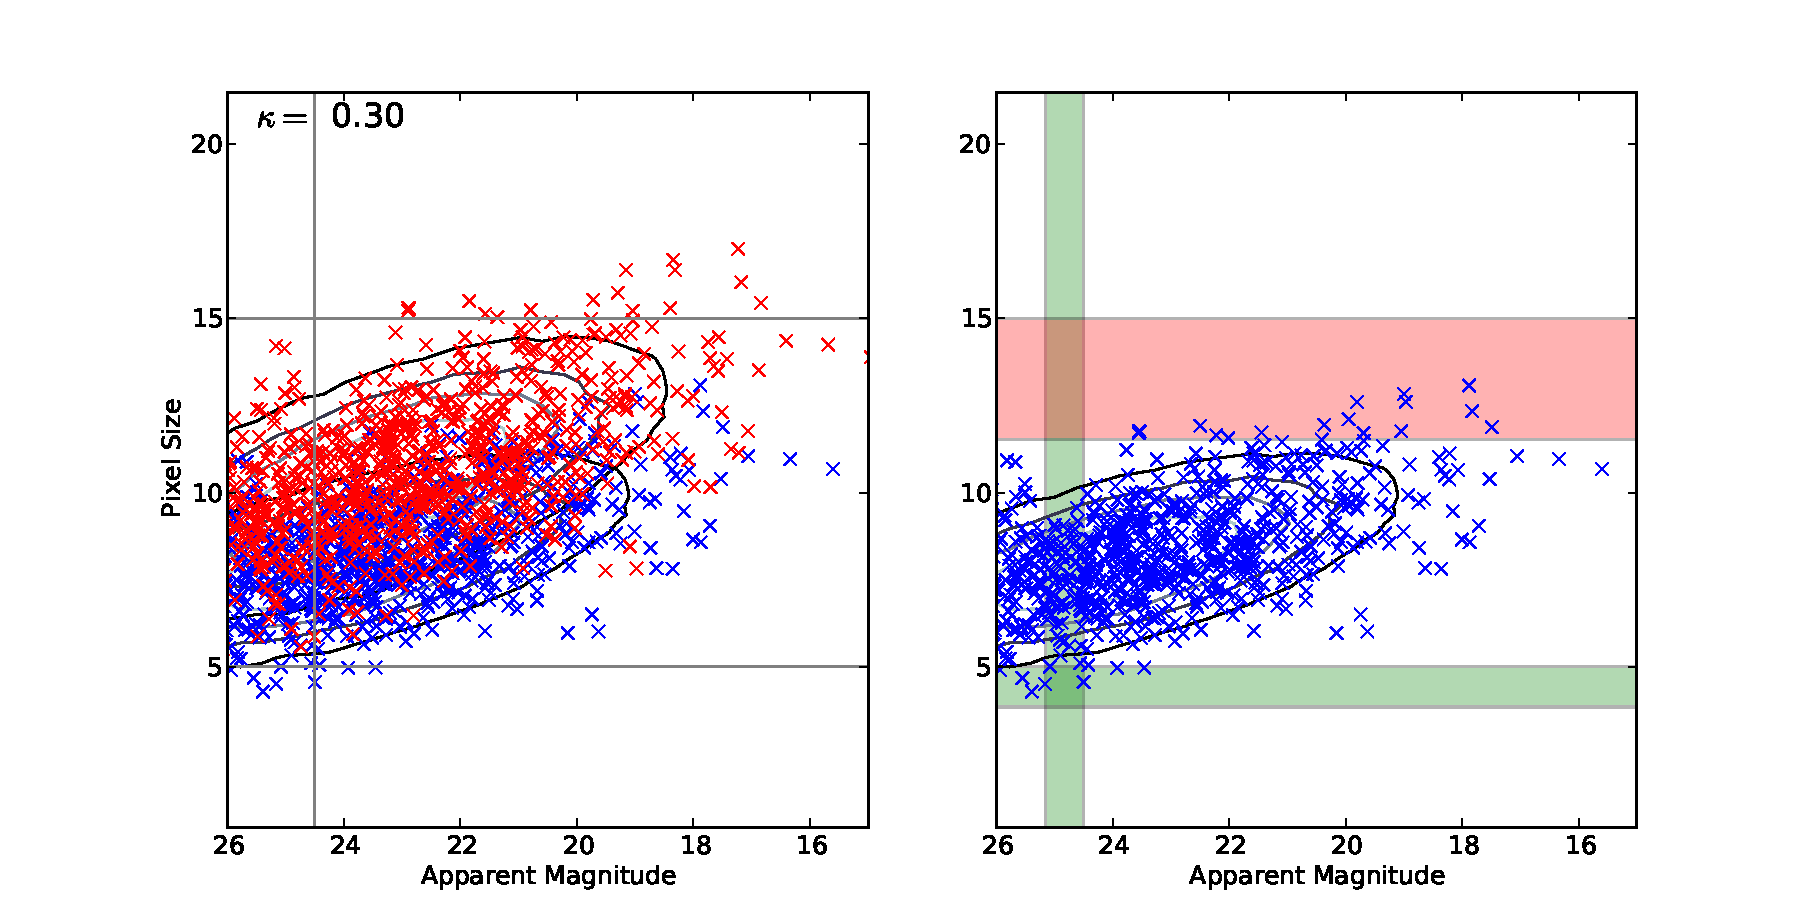
\includegraphics[width = 0.8\textwidth]{Figures/Size_Magnitude_Lensing_Diagram.pdf}
\caption{Illustrative figure showing the effect of lensing on a body of sources whose sizes and magnitudes are sampled from a multivariate Gaussian. Blue crosses correspond to unlensed sources, whilst red crosses ({\it left} panel only) show lensed counterparts. A constant convergence field of $\kappa = 0.3$ is applied. The {\it right} panel shows the equivalent local change in survey size and magnitude limits: red areas show regions of parameter space now unobservable on the lensed patch of sky, whilst green areas show regions only observable due to the action of the local convergence field. Sources in the red(green) patch are therefore removed(added) to the observed source sample.}\label{fig:Size_Mag_Lensing_Example}
\end{figure*}

\subsection{Bayesian Mass Profile Reconstruction}\label{sec:Reconstruction_Method}
%Note: ``azimuthally averaging the magnification where a spherically symmetric lens mass profile is assumed'' will likely be inaccurate where the centroid of the lens distribution is misplaced - relaxed by applicability of Bayesian method to single-source


\subsection{A joint size- and flux- magnification analysis}

Consider a single observation of the size and magnitude ($\theta, m$) of a lensed source, from which we want to place constraints on the mass profile of the lensing medium. In Bayesian nomenclature, we wish to construct a posterior distribution for a set of parameters which define the cluster mass profile (hereafter denoted using $\alpha$) from an observation of lensed quantities. Applying Baye's thereom, this can be formulated as
\be\label{eqn:BayesTheorem}
p(\alpha|\theta, m) = \frac{p(\theta, m|\alpha)p(\alpha)}{p(\theta,m)} \propto p(\theta,m|\alpha).
\ee
The `likelihood' $[p(\theta, m|\alpha)]$ describes the probability of making such an observation given a model for the lensing mass profile, and prior knowledge on the cluster mass profile may be set using $p(\alpha)$. In the last step, a flat prior was assumed on cluster profile parameters, and the evidence $[p(\theta,m)]$ is taken as a normalising constant. The implications of such as choice will be described in more detail later.

The likelihood can be related to intrinsic quantities by marginalising over these quantities as nuisance parameters
\bea
p(\theta, m|\alpha) &=& \int dm_0\;d\theta_0\;dz\; p(\theta, m|\alpha, \theta_0, m_0, z)\nonumber\\
&\times&p(\theta_0, m_0, z|\alpha),\\
& = & \int dm_0\;d\theta_0\;dz\; p(\theta, m|\alpha, \theta_0, m_0, z)\nonumber\\
&\times&p(\theta_0, m_0|\alpha)p(z|\theta_0,m_0,\alpha), \label{eqn:Likelihood_FirstExpansion}
\eea
where Baye's theorem has been reapplied to restate the final term. The final line relates the joint distribution of intrinsic size, magnitude and measured redshift to a realisation of the lensing foreground. The intrinsic size and magnitude are intrinsic to the galaxy being observed, and are therefore taken to be independent of the lensing foreground so $p(\theta_0, m_0|\alpha) \to p(\theta_0, m_0)$ and $p(z|\theta_0,m_0,\alpha) \to p(z|\theta_0,m_0)$. By enforcing this simplification, one assumes that their are no intrinsic size-, magnitude- nor redshift-density correlations which could cause a general change in size or magnitude of a population of sources physically close to the lens. This assumption should give accurate results if the source sample is selected to be radially distant from the lens so that the lensing effect dominates, however such separation is not always possible, particularly if the redshift is unknown for a large fraction of the source sample. The investigation of such correlations is outwith the scope of this work, however one may note that given a suitable model for this relation, one can naturally incorporate this model into the intrinsic size-magnitude relation by keeping the $\alpha$ dependence of this term explicit. 

Where the intrinsic size, magnitude and redshift of the source are known, the final line is described by a product of Dirac Delta functions centred on the these values. In this case, the integration is trivial, and the magnification factor associated with that lens-source system is well known. In practice, such quantities are not observable, and without prior knowledge of the true intrinsic quantities for that source one must instead marginalise over a distribution which is assumed to be known a-priori. This distribution must be representative of the source sample considered, and therefore accurately reflect the selection criteria in producing the source sample being considered to ensure parameter values are unbiased: for example, where the sample is considered in a tomographic redshift bin, the redshift distribution should reflect this choice. The extension to tomographic samples is trivial, however this comes with the caveat that the formalism presented here assumes that the redshift distribution is that of the {\it true} redshift for the sample: where an uncertainty is associated with the measured redshift, this can be incorporated by expanding out the final term as $p(z|\theta_0,m_0) \to \int d\hat{z} p(z|\hat{z}, \theta_0, m_0)p(\hat{z}|\theta_0, m_0)$, where $\hat{z}$ denotes the measured redshift and the uncertainty in this measure can be incorporated in the former term in this expansion. Similar expansions may be used when there is an uncertainty in the measured quantity of interest (for example with measurement noise in size or magnitude determination), however for simplicity it is assumed that such considerations are negligible in the remainder and are ignored unless otherwise stated. As such, for the remainder of this section we assume that measurement noise is sub-dominant to intrinsic variations in the measured quantity.

In the absence of measurement noise, the former term in equation \ref{eqn:Likelihood_FirstExpansion} contains information on the lensing of the source and can be determined using the relations given in Equations \ref{eqn:Lensing_Relations__Size} to \ref{eqn:Lensing_Relations__Flux} as
\bea\label{eqn:Observed_Intrinsic_SizeMagnitude_Relation}
p(\theta, m|\alpha, \theta_0, m_0, z) &=& \delta_D(\theta - \theta_0\mu^{\frac{1}{2}}[\alpha,\xi,z])\\
&\times&\delta_D(m - m_0 +2.5\log_{10}\{\mu[\alpha,\xi,z]\}),\nonumber
\eea
where $\xi$ densities the physical transverse separation of the lens and source. Using a change in variables, the marginalisation over the intrinsic size and magnitude can be carried out so that the posterior takes the form
\be\label{eqn:Size-Magnitude_SMD_Posterior}
\begin{split}
p(\theta, m|\alpha) =  &\int \;dz \mu^{-\frac{1}{2}}p_{[\theta_0,m_0| z]}\left(\mu^{-\frac{1}{2}}\theta,m+2.5\log_{10}\{\mu\}\right)\\
& \times \; p_{[z|m_0, \theta_0]}(z| m+2.5\log_{10}\{\mu\}, \mu^{-\frac{1}{2}}\theta),
\end{split}
\ee
where notation $p_{[x]}(y)$ denotes the probability density function for $x$ evaluated at $x=y$. The likelihood for each galaxy is then constructed by sampling the intrinsic size-magnitude distribution along a `de-lensing' line. Thus, with knowledge of the intrinsic size-magnitude and redshift distribution for the source sample, one can obtain constraints on the mass profile parameters of the lensing system for a single source. In principle, these distributions can be measured directly using data taken over a blank field, or a large survey area. 

The posterior on lens mass profile parameters can then be constructed for a single source by reapplication of Baye's Theorem (as in equation \ref{eqn:BayesTheorem}), and joint constraints using the whole source sample can be obtained by multiplying single-source posteriors (or summing log-posteriors) in the usual way.

\subsection{Correct normalisation of the likelihood}

Whilst equation \ref{eqn:Size-Magnitude_SMD_Posterior} gives the posterior for dark matter profile parameters using magnification measurements, the formulation presented is only correctly applicable to the special case where no cuts on size or magnitude are applied to the data. In such a case, the correct normalisation of the posterior according to the evaluation of the evidence is a trivial exercise, equivalent to an overall shift in the amplitude of the posterior.

Such a situation is unlikely in the application to real data, where consideration on the fidelity and completeness of the source sample may be questionable on certain scales, for example for small or faint sources. It is therefore likely the that source sample is chosen using some selection function dependent on magnification dependent quantities such as the measured size and magnitude, and this must be taken into account in the evaluation of the posterior to avoid inaccurate parameter measurements. Where hard magnitude and size cuts are applied in the source sample selection, the application of a non-zero magnitude factor will shift the true underlying intrinsic size-magnitude distribution in the size and magnitude planes, altering the normalisation of the likelihood (see Figure \ref{fig:Size_Mag_Lensing_Example}). In this case, the posterior must be normalised such that
\be
\int^{m_u}_{m_l} {\rm d} m \int^{\theta_u}_{\theta_l} {\rm d}\theta \; p(\theta,m|\alpha) =  1
\ee
where the integrals are understood to extend over {\it lensed} quantities. By substituting the form of the posterior in equation \ref{eqn:Size-Magnitude_SMD_Posterior} and assuming an deterministic relationship between the measured size and magnitude and their unlensed counterparts, the magnification-dependent nature of the normalisation can be made more explicit:
\begin{widetext}
\bea
\int dz\; \mu^{-\frac{1}{2}} \int_{m_l}^{m_u} dm\int_{\theta_l}^{\theta_h} d\theta\; p_{[\theta_0, m_0|z]}\left(\mu^{\frac{1}{2}}\theta,m+2.5\log_{10}\{\mu\}\right) p_[z|m_0,\theta_0](z|m+2.5\log_{10}\{\mu\}, \mu^{\frac{1}{2}}\theta), \nonumber\\
= \int dz\; \int_{m_l+2.5\log_{10}\{\mu\}}^{m_u+2.5\log_{10}\{\mu\}} dm_0\int_{\mu^{-\frac{1}{2}}\theta_l}^{\mu^{-\frac{1}{2}}\theta_h} d\theta_0\;p\left(\theta_0,m_0\right)p(z|m_0, \theta_0) = 1. \nonumber
\eea
\end{widetext}
The normalisation is then seen to vary with magnification factor, and consequently with the set of cluster mass profile parameters ($\alpha$) for a given source. In contrast to the case where no cuts are applied, such a normalisation will change the shape of the recovered posterior, and thus neglecting this effect is likely to bias recovered cluster profile parameters.

Here, I have considered only hard cuts on the data, however in reality it may often be the case that a smooth selection function is applied to the data. Such a case is considered in more detail in \cite{Alsing:2014p2846} and can be easily extended to the analysis presented here where the form of the selection function is known. For the remainder of this paper, I consider only the case where hard cuts are applied to the data, as detailed here.

\subsection{Analysis using sizes or magnitudes only}\label{sec: Size_Magnitude_Only_method}

In the preceding sections, I have presented a method for obtaining constraints on lens mass profile parameters using a joint analysis of source size and magnitude information using the magnification effect. In certain circumstances, one may wish to consider either of these  measurements independently. When this is done, information is removed from the analysis and statistical errors on inferred parameter constraints would be larger, however removing such a measurement may remove potential bias where the measurement is systematically incorrect. 

In the type of analysis motivated in this paper, one may wish to ignore size measurements for the smallest sources where the effect of optical distortions may introduce large systematics in the measurement, or where the assumption of negligible measurement error in galaxy size is least valid, but for whom the measured magnitude is considered more robust. Where this is the case, the source sample can then effectively be split into two independent samples: for one, a full, joint size plus magnitude analysis is used to produce mass parameter constraints, whilst for the other an analysis using only magnitude measurements is taken. Each sample represents an independent measurement of the lens mass profile, and the resultant posteriors can be combined to minimise the statistical error in the final analysis.

Where only reliable magnitude information is available, posteriors may be produced by marginalising the likelihood given in equation \ref{eqn:Size-Magnitude_SMD_Posterior} over the full range of source sizes considered in the sample
\begin{flalign}
&p(m|\alpha) = \int dz\; \mu^{-\frac{1}{2}} \int_{\mu^{-\frac{1}{2}}\theta_l}^{\mu^{-\frac{1}{2}}\theta_u} d\theta_0\\
&\times p_{[\theta_0, m_0]}\left(\theta_0,m+2.5\log_{10}\{\mu\}\right) p_{[z|m_0,\theta_0]}(z|m+2.5\log_{10}\{\mu\},\theta_0),\nonumber
\end{flalign}
where $\theta_l$ and $\theta_u$ denote the size limits of the source sample, and where
\be 
\int^{m_u+2.5\log_{10}\{\mu\}}_{m_l+2.5\log_{10}\{\mu\}} {\rm d}m_0 \; p(m_0|\alpha) = 1
\ee
where $m_u$ and $m_l$ represent the limits of the observed magnitude for the sample. The intrinsic magnitude distribution ($p_{[m_0]}$) must be representative of the galaxy sample, and must account for intrinsic size-magnitude correlations where the sample considered is size-limited. In the final relation, I have again assumed a deterministic, lensing-only relation between observed magnitude and intrinsic magnitude, to make the magnification-factor-dependent nature of the normalisation explicit.

Similarly, a size-only posterior may be formed by marginalising over the lensed magnitude, giving 
\bea\label{eqn:Size-Only_SMD_Posterior}
p(\theta|\alpha) &=& \int dz\; \mu^{-\frac{1}{2}} \int_{m_l+2.5\log_{10}\{\mu\}}^{m_u+2.5\log_{10}\{\mu\}} dm_0\;\\
&\times& p_{[\theta_0, m_0]}\left(\mu^{-\frac{1}{2}}\theta,m_0\right)p_{[z|m_0,\theta_0]}(z|m_0, \mu^{-\frac{1}{2}}\theta).\;\;\;\;\nonumber
\eea
with 
\be
\int^{\mu^{-1/2}\theta_u}_{\mu^{-1/2}\theta_l} {\rm d}\theta_0 \; p(\theta_0|\alpha) = 1.
\ee

\subsection{Extension to Ellipticities}

Where ellipticity information is also available, the above formalism can be extended to construct a joint shear and magnification analysis of the lens mass profile. Such a combination has be the focus of a slew of current research, %DIscussion on advantages of this, Rozo etc.

Following the previous method, the likelihood can be constructed by integrating over intrinsic quantities as nuisance parameters
\bea
p(\theta, m, e|\alpha) &=& \int {\rm d}z \; {\rm d}\theta_0 \; {\rm d}m_0 \; {\rm d}^2e_0 \; p(\theta, m, e|\alpha, \theta_0, m_0, e_0, z)\nonumber\\
&\times& p(\theta_0,m_0,e_0)p(z|\theta_0,m_0,e_0)
\eea
where $e$ denotes both ellipticity components in a given co-ordinate frame. As before, the second term gives the redshift distribution of the population form which the source was a sampled, and any redshift dependence of the intrinsic ellipticity, size of magnitude can be incorporated into this term. The first term in this equation gives the relation between the observed quantities and the intrinsic quantities, which is assumed to be deterministic and solely due to lensing in the limit of negligible measurement errors\footnote{As previously, this assumption can be relaxed by marginalising over an intermediary estimator which denotes the true lensed quantity: for example, in the case of a the ellipticity, one can consider $p(e|e_0,\alpha,z) \to \int d^2\hat{e} \; p(e|\hat{e})p(\hat{e}|e_0,\alpha, z)$, where the latter relation contains the lensing information, and the former the uncertainty in the measured estimate of the lensed ellipticity.}
\begin{flalign}
p(\theta, m, e|&\alpha, \theta_0, m_0, e_0, z) = \delta_D(\theta - \theta_0\mu^{\frac{1}{2}}[\alpha,\xi,z])\nonumber\\
&\times\delta_D(m - m_0 +2.5\log_{10}\{\mu[\alpha,\xi,z]\})\nonumber\\
&\times\delta_D(e - \mathcal{E}[e_0,g])
\end{flalign}
where $\mathcal{E}$ denotes the action of the lensing reduced shear on the nuisance intrinsic ellipticity parameter considered, such that $\mathcal{E}^{-1}(e,g) = e_0$ and $\mathcal{E}(e_0,g) = e$. In the weak lensing limit, the observed ellipticity may be related to the intrinsic ellipticity of the source and the applied shear field by way of a Taylor Expansion
\be
e_{\alpha}(e_0,g) = e^{\alpha}_0 + \frac{\partial e_{\alpha}}{\partial g_{\beta}}g_{\beta} + O(|g|^2) = e^{\alpha}_0 + P^{\gamma}_{\alpha\beta}g_{\beta},
\ee
where the coefficient of the linear term is frequently referred to as the `shear responsively', and details how the measured ellipticity responds to the applied shear field. In the parlance used here, this can be expressed as
\bea
\mathcal{E}_\alpha = e^{\alpha}_0 + P^{\gamma}_{\alpha\beta}g_{\beta}\nonumber\\
\mathcal{E}^{-1}_\alpha = e^{\alpha} - P^{\gamma}_{\alpha\beta}g_{\beta}\nonumber.
\eea
Similar expressions can be determined where ellipticities are defined using quadrupole measurements on images, where the weak lensing limit has not been applied, as in \citep{Seitz:1995p2763,Seitz:1997p2784}.

The posterior is then given by
\bea
p(\theta, m, e|\alpha) &=& \int {\rm d}z \left(\prod_{i=1}^2 \frac{\partial \mathcal{E}^{-1}}{\partial e_{i}}\right) \; p(\mu^{-\frac{1}{2}}\theta,m+2.5\lg10{\mu},\mathcal{E}^{-1})\nonumber\\
&\times& p(z|\mu^{-\frac{1}{2}}\theta,m+2.5\lg10{\mu},\mathcal{E}^{-1}).
\eea
When ellipticity measurements only are considered, this can be reduced to 
\be
p(e|\alpha) = \int {\rm d}z  \left(\prod_{i=1}^2 \frac{\partial \mathcal{E}^{-1}}{\partial e_{i}}\right) \; p(\mathcal{E}^{-1})p(z|\mathcal{E}^{-1})
\ee
and the posterior for the source sample constructed as before. 
%Discussion of mass sheet degeneracy as cluster parameter,shear measurement methods as \mathcal{E}^{-1}, and independent measures, normalisation.

\subsection{Advantages and Caveats}

%-- This method is not immune to the bias due to inaccuracies in the intrinsic distributions
%-- No need to fit an NFW to stacked lenses: instead constraints on NFW can be placed for a single lens system and posteriors for a multiple lens system can be combined.

In the previous sections, we have motivated a way to produce full posterior distributions of cluster parameter values based on the assumption of an underlying mass profile model which can be related to lensing observables, and a-priori knowledge of the intrinsic size-magnitude distribution. The main strengths in utilising such a techniques lie in the flexibility of the method: complications and extensions can be easily added through explicit marginalisation of latent variables provided they can be related to the observables and intrinsic quantities, and this is done explicitly in the marginalisation over a a-priori redshift distribution.

The use of a-priori distributions means that the method can be easily implemented using well-motivated theoretical models, or using measurements from the data where available. As such, the application can be entirely self-consistent. However, where the model is measured from data, one must be aware that noise or systematic uncertainties in the measurements can enter the analysis through their affect on the a-prior distributions themselves. Where this is the case, only systematic errors in the measured intrinsic quantities which vary with density of in a spatially dependent way will be problematic, as constant offsets across the whole field will cause a identical shift in the a-priori distributions and the sample provided they are both equally affected, and will not affect the recovered mass profile parameter interpretation. Noise in the measured distributions can be dealt with by smoothing, or fitting a theoretically motivated model to the data.

The application of this method will focus on the mass profile reconstruction of individual over-densities in the remainder of this paper, but a particular advantage of the use of this method is the fact that posteriors can be constructed individually for each source, and individually for each foreground lens before further combination. As such, for an analysis which aims to maximise signal--to--noise by stacking lenses, the application of this method allows one to fit the chosen mass profile model to each lens individually and produce model parameter constraints for the lens sample by combining these posteriors in the usual way. This therefore avoids the need to fit a mass profile to the stacked measurement, whose shape can be affected by systematics in each individual lens measurement, for example in smearing out the profile towards the centre caused by mis-centering on each lens of the stack.

In the application of this method, we choose to work with full recovered model parameter PDFs until the final stage where a maximum-posterior estimator is used to visualise the results in different contexts. Doing so increases the run-time over the case where statistics are formed from frequentist estimators based on the statistical measures of the source sample. Especially in the case where multiple latent variables are marginalised over, this can be computationally expensive in comparison, however we note that recent work in advanced statistical techniques such as Hierarchical Bayesian Inference \citep[e.g.][]{2015arXiv150507840A,2015ApJ...807...87S} and advanced sampling methods can go some way to reducing the necessary run-time.

\section{The STAGES dataset}\label{sec:STAGESDataset}

The STAGES survey \citep{Gray:2009p2720} utilised the F606W filter of the Advanced Camera for Surveys ({\it ACS}) of the Hubble Space Telescope ({\it HST}) to image a quarter square degree centred on the A901/2 supercluster. STAGES images are complimented by optical imaging using COMBO-17 \citep{Wolf:2003p2805} with five broad bands and twelve narrow bands, and which provides high quality photometric redshifts, with the precision $\sigma_z \sim 0.02(1+z)$ for about $\sim 10\%$ of the brightest galaxies ($R_{\rm Vega}<24)$ in the STAGES sample. The survey provides deep ($m_{\rm F606W} \lesssim 27.5$), high resolution HST images of $\sim 70,000$ extended sources, from which one can expect that a large sample set of robust galaxy shapes, sizes and fluxes can be obtained. The observational footprint of the survey covers $\sim 0.22$ square degrees, giving a global number density of sources of $\sim 85 \; {\rm gal/arcminute}^2$ using the whole sample of extended sources. Observations were taken within a small observational time frame, with greater than $50\%$ of the tiles were observed in one five-day period, and over $90\%$ within 21 days, whilst seven tiles were observed six months later.  The mosaic of 80 ACS tiles which constitutes the STAGES field is shown in \cite{Heymans:2008p2060}, grouped in colour by observation period, and covers a total area of $\sim 823$ square arc-minutes, accounting for masking.

The Galaxy Evolution and Morphology Survey (GEMS) \citep{Rix:2004p2800} observed a quarter square degree blank field in 9x9 pointings in MF606W using ACS. As with the STAGES field, HST images of the GEMS field are complemented by imaging from COMBO-17 for galaxies with $R<24$, providing accurate redshifts for $\sim 10,000$ galaxies in the GEMS sample. This combination of a high number density of sources with high resolution imaging and complementary GEMS dataset from which intrinsic size and flux properties may be obtained provides quality dataset on which to study the use of source magnification as a proxy for cluster mass estimation. Whilst the GEMS dataset provides the means to estimate the distribution of intrinsic sizes and magnitude of field galaxies, which can directly feed into the analysis presented here, the construction of the prior using the lensed STAGES dataset is shown to produce only small bias in Section \ref{sec:ApplicationToMocks}, and is therefore considered negligible in this study.

The application of the method to the STAGES data provides a unique set of idiosyncratic complications. The biggest complication comes from the lack of redshift information for approximately $90\%$ of the source sample. This affects the analysis as presented in two ways: firstly, the lack of multi-band photometry for this sample complicates the removal of cluster members, detailed further in the next section; and secondly, without redshift information we must marginalise over an a-priori redshift distribution for the sources to convert lensing observables to cluster mass profile parameters. Following the shear application in \cite{Heymans:2008p2060}, we model the a-priori redshift distribution as 
\be\label{eqn:RedshiftDist}
p(z|m) = \frac{\beta}{z_0\Gamma \left( \frac{1+\alpha}{\beta} \right)}\left(\frac{z}{z_0}\right)^\alpha e^{-(z/z_0)^\beta}
\ee
with $z = z_{\rm median}/1.412$, $\alpha = 2$, $\beta = 1.5$ and using the median-redshift magnitude relation of \cite{Schrabback:2007p2802}
\be\label{eqn:zmed_mag}
z_{\rm median} = 0.29[m_{\rm F606W} - 22] + 0.31.
\ee

\subsection{Mass Profile Modelling}

%NFW
%Possible free parameters
%M-c relation
%Aim: to compare to shear

We take the mass profile of the lensing clusters to be spherically-symmetric NFW profiles \citep{Navarro:1997p2675}, and relate the profile parameters to lensing parameters using the analytic relations of \cite{Wright:2000p2260}. The base model profile is a function of four parameters, namely the position of the centre of the profile (centroid), the redshift of the lens, the virial radius/virial mass and the concentration. With the exception of CB1 at $z = 0.46$ \citep{Taylor:2004p2808} all lenses are placed at a fixed redshift $z = 0.165$ \citep{Gray:2009p2720}. Following the shear analysis, we use the mass-concentration relation of \cite{Dolag:2004p2721}, and take the cluster centre positions to be those quoted in \cite{Heymans:2008p2060}. As a result, the NFW fit is a function only of the virial mass/virial radius for the remainder of this text. Whilst we note that more recent mass-concentration relations exist, and emphasise that the centroid position and concentration cold be simultaneously fit using this method, the over-riding aim of this analysis to to compare cluster profile estimates between the shear and magnification analyses, and so we choose to set up the analysis using the same assumptions as \cite{Heymans:2008p2060} to facilitate comparison.

\subsection{Source Selection}\label{sec:Source_Selection}

The method is applied to the source catalogue used in the analysis of \cite{Heymans:2008p2060} (hereafter referred to as CH), matched to the publicly available STAGES catalogue \cite{Gray:2009p2720} (hereafter ST). The CH catalogue consists of $79,366$ sources ($n_{\rm gal} = 96.5$ sources per square arcminute) with magnitude information, whilst the ST catalogue contains a total of $46,471$ sources ($n_{\rm gal} = 56.5$ with SExtractor and GALFIT size and magnitude information, as well as COMBO-17 redshift estimation for $10,790$ sources after matching. A preliminary investigation (detailed further in Appendix \ref{sec:STAGES_RRG_Measurement}) suggests that the use of model-fitting methods will provide a more accurate size determination for low surface brightness sources, where non-parametric measures such as quadrupole moments or aperture sizes cannot distinguish between faint, large galaxies and bright, small galaxies. The final source sample therefore consists of the SExtractor magnitude information (MAG\_BEST) as given in the CH catalogue, chosen to give the largest source sample with magnitude information, with GALFIT scale radius used as the source size measured, where available. The size and magnitude distributions across the field, after subtracting conservative $3$ arc-minute apertures around the BCG cluster centres to remove cluster members, is given in Figure \ref{fig:SizeMag_Distribution_Master}, and forms the a-priori distribution for this analysis.

The bottom panel of Figure \ref{fig:SizeMag_Distribution_Master} shows the marginalised magnitude distribution between the CH and ST catalogues. One can see that the marginalised magnitude distribution for the CH catalogue extends to fainter magnitudes than the public ST catalogue, reflecting the differing selection of the source sample, where the catalogue of CH reflects the choice to include smaller and fainter samples in the shear analysis of \cite{Heymans:2008p2060}.

%%Notes on the size distribution and comparison to published results (Shen, Lani, Alsing).
\begin{figure*}
\centering
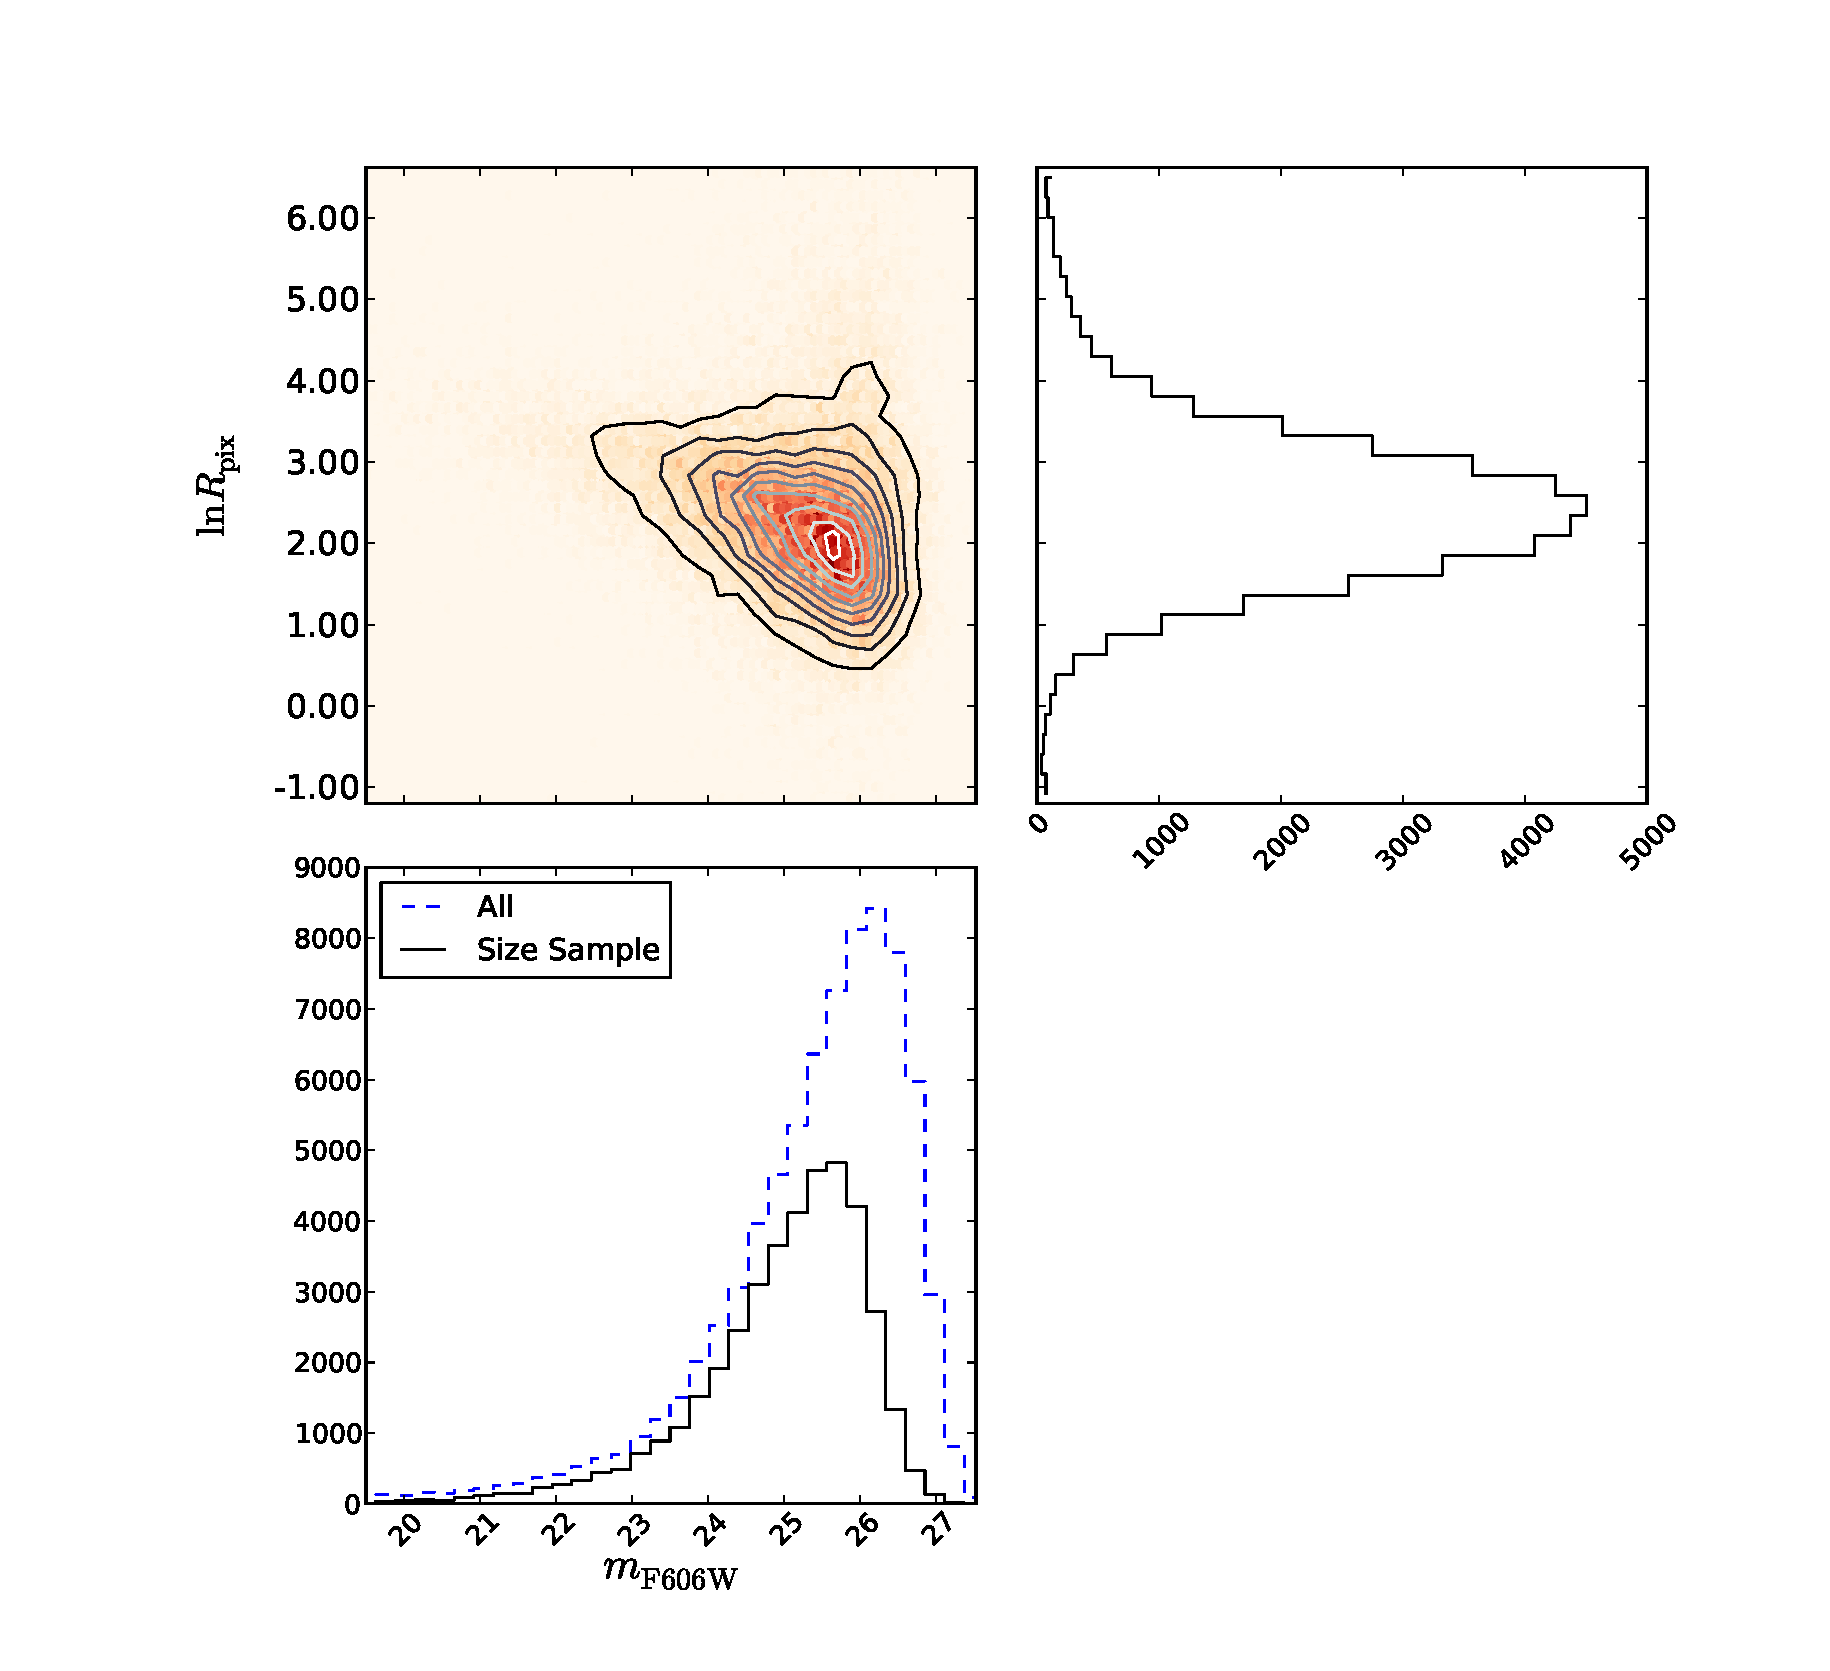
\includegraphics[width = 0.9\textwidth]{Figures/Data/Distributions/STAGES_Size-Mag_Distribution_withRRGMagComp.pdf}
\caption{The joint size magnitude (upper left) and marginalised size (upper right) and MF606W magnitude (lower) distributions used to for the a-priori size-magnitude distribution. Black solid lines show the distributions obtained from the sources in the matched CH and ST catalogues, whilst the blue dashed line shows the magnitude distribution for the CH catalogue only} \label{fig:SizeMag_Distribution_Master}
\end{figure*}


%General selection and source split
Sources are selected in $3'$ apertures around the cluster BCG, taken from Table 1 of \cite{Heymans:2008p2060}. The source sample is further split into two independent samples: the first contains those sources for whom a reliable source size is available and is used for a full joint size-magnitude analysis; the second corresponds to those sources for whom size information is either unavailable or considered unreliable and is therefore considered only as part of an analysis using measurements of source magnitude only. In all cases a lower size cut of $\ln R = 0.78$ is used to remove the smallest sources for whom the correction of the PSF is least robust, and are considered only as part of the second sample. This corresponds to a cut of $R < 2.2$ pixels, which is equivalent to the cut used in \cite{Schmidt:2012p1106}.

Unless otherwise stated, the final result is presented as the combination of a joint size-magnitude measure for the sources with both size and magnitude information available (sample 1) with a magnitude-only analysis for the remaining sample (sample 2). 

%Magnitude and redshift cuts
The inadvertent inclusion of cluster members in the source sample can introduce a bias in the derived cluster model parameters, as they are mistakenly interpreted as lensed sources in the analysis. The result of the inclusion of cluster members is further complicated in the presence of an intrinsic size-density correlation, which is unaccounted for in the analysis. This is a particular problem in the application to the STAGES dataset, as COMBO-17 redshift information is only available for $\sim 10\%$ of the sample, meaning a simple redshift cut is unlikely to remove all cluster members from the sample. We apply a redshift cut of $z<0.2$ on sources where redshift information is available, and a bright magnitude cut of $m<23$, corresponding to a median redshift of $z=0.6$ in the median-redshift-magnitude relation of equation \ref{eqn:zmed_mag}, following \cite{Heymans:2008p2060}. The lower panels of Figure \ref{fig:magDiff_byMeasure} show the number density contrast of sources in annular bins around the BCG for each of the four main clusters considered, after the application of redshift and magnitude cuts on the sample. One can see that even after the application of such cuts, the number density of sources is higher than the field average towards the centre of the cluster, most noticeably for A901b and SW, with an amplitude larger than can be accounted for from magnification bias alone.  This suggests that the applied bright magnitude and redshift cuts are insufficient to fully remove cluster members. 

The top panels of figure \ref{fig:magDiff_byMeasure} shows the difference between the mean magnitude in radial bins around the BCG of each cluster to the field mean (after the masking of the four clusters) as a function of varying faint limiting magnitude of the source sample, with plots of the number density contrast in radial bins. As such, each magnitude difference can be related to average magnification factor for sources within that annulus, however one must note that this measure has not been corrected for the application of size and magnitude cuts, and is therefore not an unbiased estimate of the cluster mass. However, the use of this estimate can give a useful diagnostic on the behaviour of the signal around the cluster centre.  One can see that, for A901a, A902 and SW the magnitude difference in radial bins is well behaved at large radii, with a general trend towards more negative values as the faint limit used is relaxed. This behaviour may be attributed to the lack of correction for the use of a magnitude cut: where a global faint cut is applied, the mean measured around a magnification field will be underestimated. By contrast, for A901b, the use of a brighter faint cut shows the opposite trend, and we see that for A901b the magnitude difference using the $m<26$  sample is discrepant with more relaxed cuts. This indicates that the signal around A901b is sensitive to the limiting magnitude, and provides a flag to the reliability of the magnitude estimation of the faint sources in that region. We note that A901b shows that largest extended X-Ray emission on the STAGES field, and consequently the reliability of the magnitude determination of the faint sources could be compromised by the presence of unaccounted-for intra-cluster light. As a result, the sources chosen around A901b are taken to be those which satisfy $m<26$. In this case, the sample of sources around A901b are considered as a separate sample to the remaining sample, and the application of a stricter magnitude cut requires that the posteriors obtained for each of these sources galaxies must be correctly normalised to account for this to avoid bias in cluster parameter estimation.  An analysis in which this cut is removed is verified to produce constraints on cluster virial radius consistent with zero, and significantly discrepant to the shear analysis of \cite{Heymans:2008p2060}.

Motivated by the trends described here, we therefore apply conservative core cuts on the sample or $1.2', 1.2', 0.5',$ and $0.9'$ around the A901a, A901b, A902 and SW BCGs respectively (shown as dot-dashed vertical lines in Figure \ref{fig:magDiff_byMeasure}). In the case of A901b the number over density of sources extends across the whole angular scale considered here suggesting that cluster member contamination may persevere in spite of the application of source removal within this aperture, however stricter cuts will remove progressively more of the source sample, and will leave only those sources furthest from the cluster centre which are least lensed and whose leaning determination is expected to be most noisy. A901a shows no significant variation in number density contrast towards the BCG, however consideration of the magnitude difference with the application of faint cuts towards the centre motivates the conservative core removal  applied here.

The application of such cuts removes a significant fraction of the sources for whom the lensing signal will be strongest, removing $402, 515, 70, 282$ galaxies from the source sample around each cluster respectively. The need to apply such strict core cuts should be considered a particular limitation of the data-set used, and it may be considered that cluster model parameter values may be constrained to higher significance in a data-set with more complete redshift information.

After the application of all the above cuts, the source sample consists of $2189, 1230, 2437, 2110$ galaxies around A901a, A901b, A902 and the SW group respectively, with $1194$ faint sources removed around A901b by the application of a faint cut of $m<26$.

\begin{figure*}
\centering
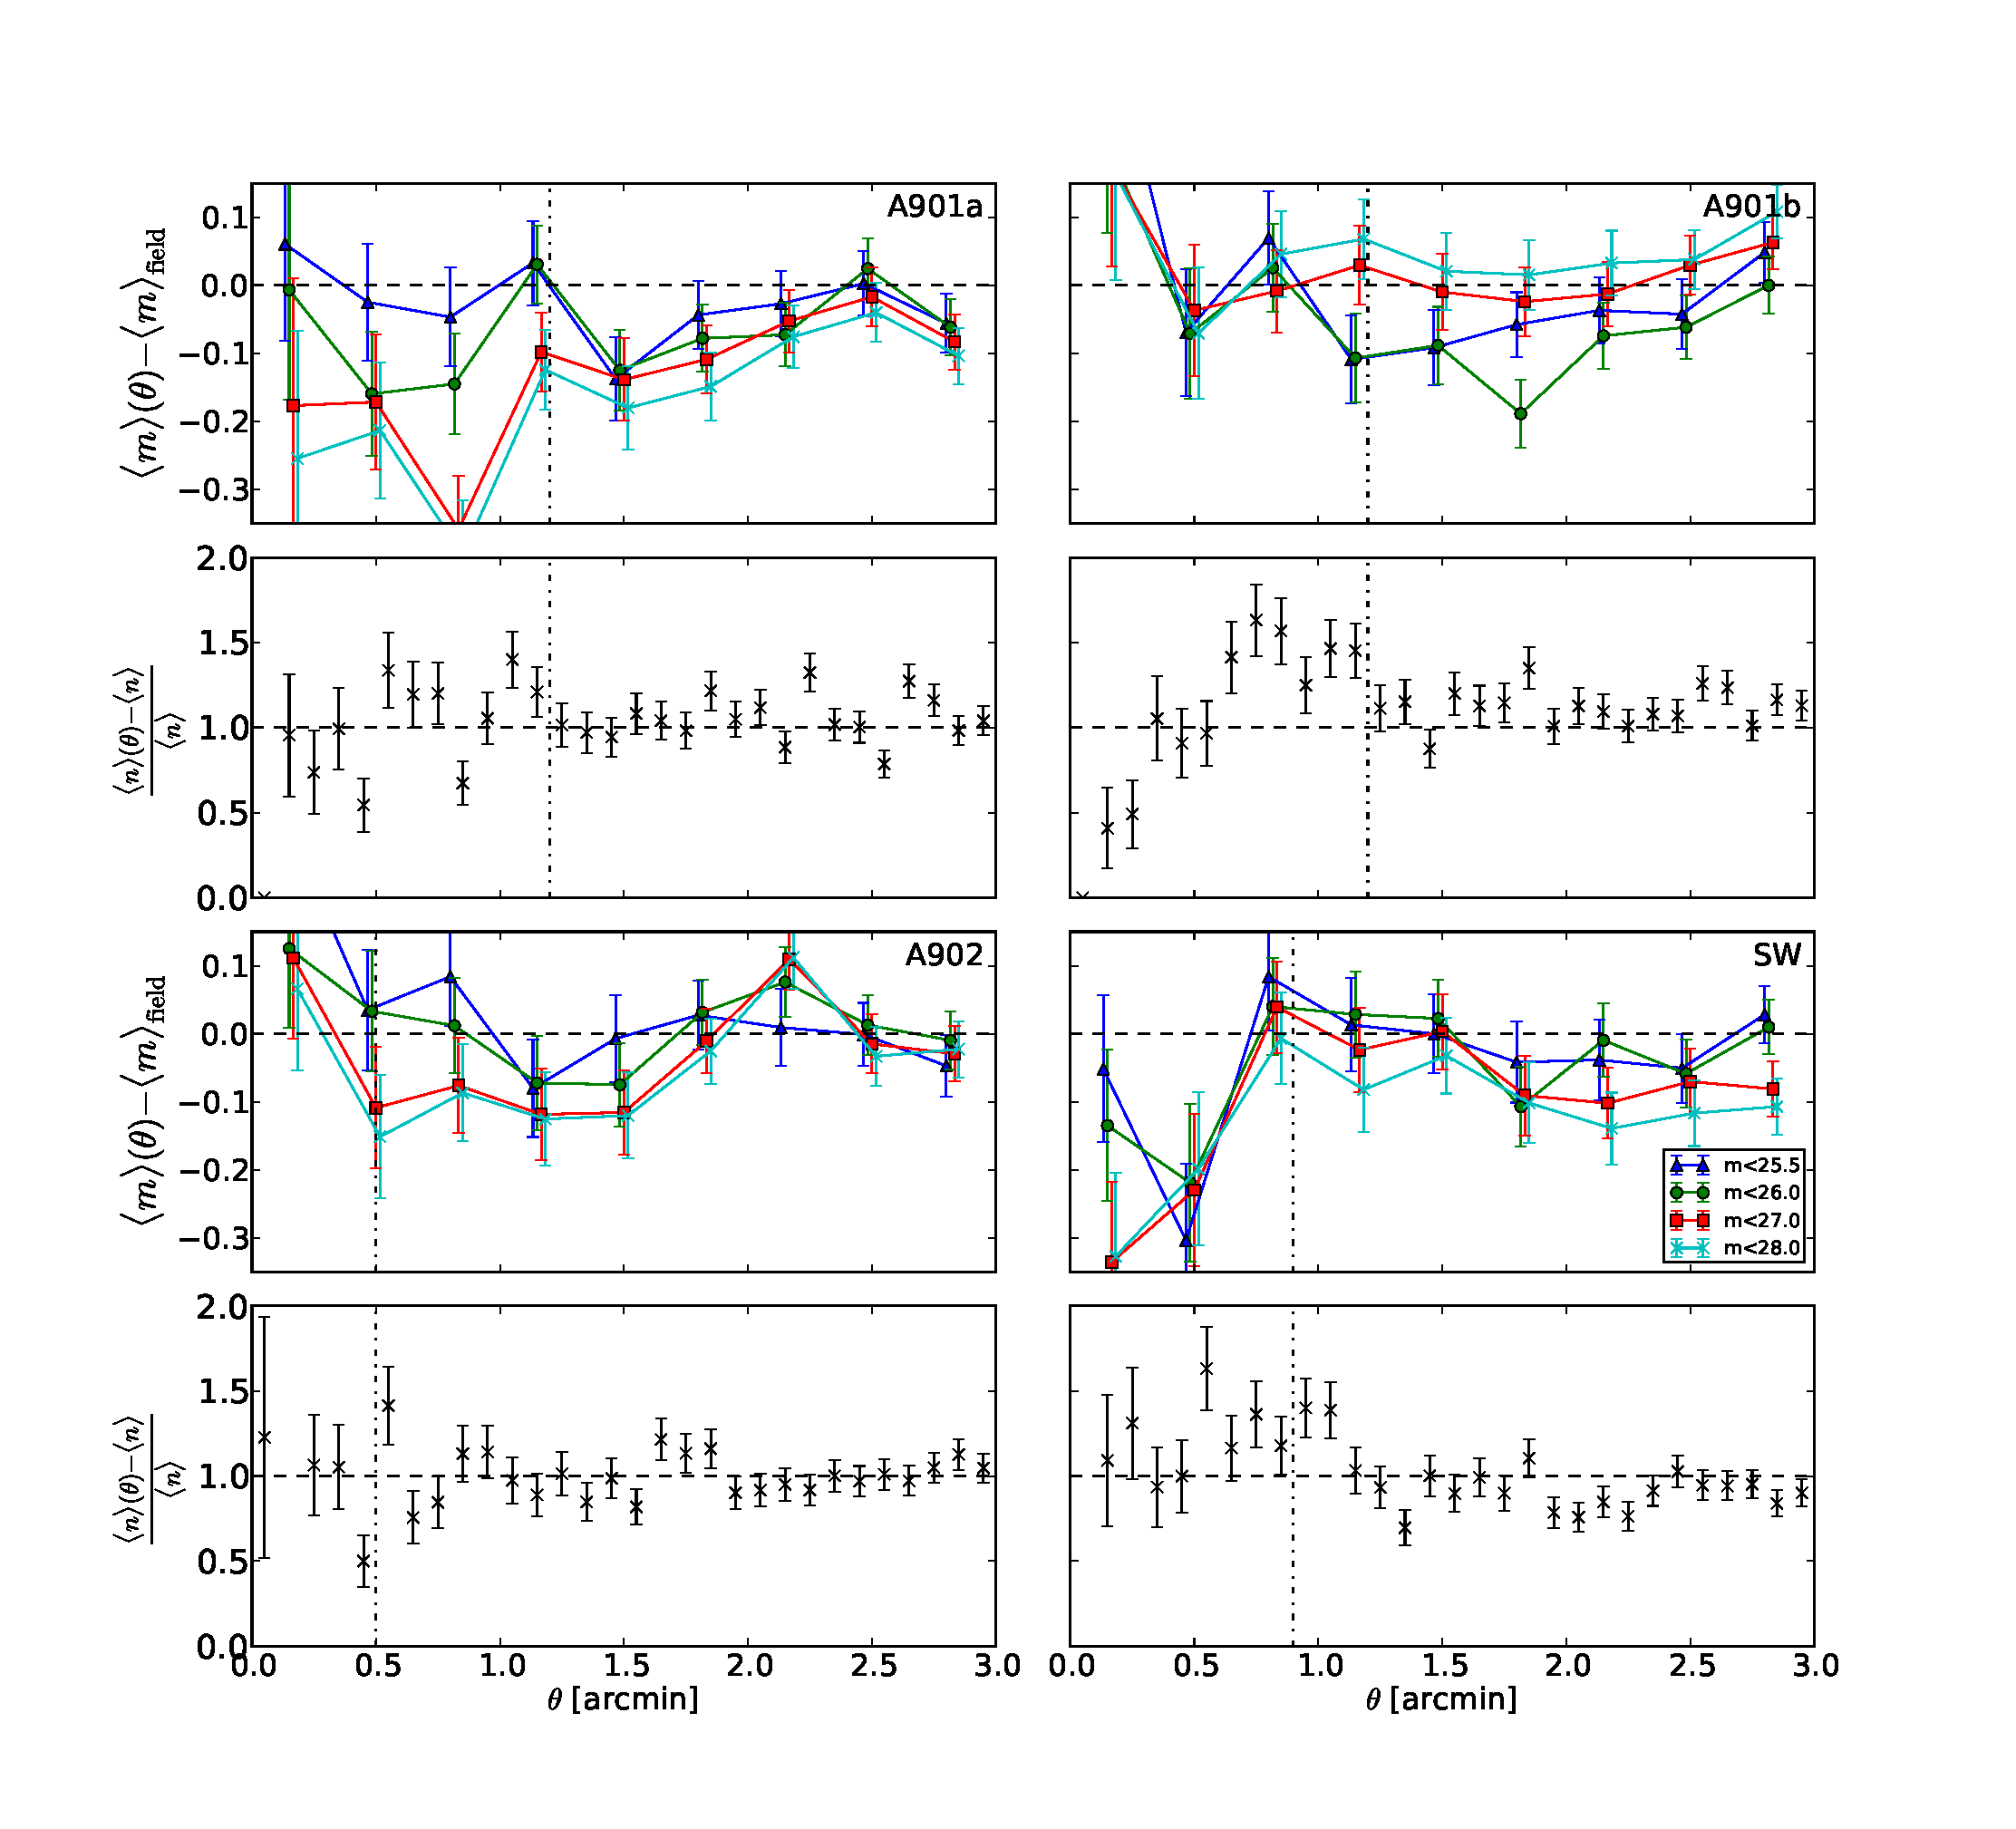
\includegraphics[width = 0.9\textwidth]{Figures/Data/magDiff_InRadialBins_CH_A901ab_A902_SW_withCC.pdf}
\caption{Plot showing the difference between the mean magnitude in radial bins from the BCG against the mean of the a-prior distribution, for A901a (top) and A901b (bottom) as a function of limiting faint magnitude.  Left plots use the magnitudes from the CH catalogue, whilst right shows the Master catalogue magnitudes. As limiting magnitude is varied, the difference around the field mean for A901b is not stable until approximately $m<26$.} \label{fig:magDiff_byMeasure}
\end{figure*}

\subsection{Alternatives to source selection criteria}

%The presence of galaxies which reside either in or in the foreground of the lensing cluster will not have experienced lensing due to the mass profile of the cluster itself, and therefore the inadvertent inclusion or a significant sample of cluster galaxies in the source sample can be expected to result in an underestimation of the magnification of the sample, and resultant cluster profile measurements. This is a particular problem for the application of this method to the STAGES data as $\sim 90\%$ of observed sources do not have redshift or multi-colour information. Whilst the application of redshift cuts, where available, and a bright magnitude cut should minimise the contamination of the sample by these bodies, the presence of cluster contaminants is expected in the final sample. Figure \ref{fig:Foreground_Contamination_Plots} shows the number density of catalogue objects around each cluster BCG, plotted against the global mean number density for that analysis, given as the number of sources in the sample after cuts divided by the survey area, accounting for masking. A902 shows an increase in the number density of sources towards the centre of the cluster, indicative of contamination of the source sample by cluster members. A901a shows a decrease in number density toward the cluster centre, indicative of foreground masking. The SW group shows an increase in number density towards small angular scales followed by a decrease. A901b shows an increase in number density over the global value on all scales, suggesting that cluster contamination for A901b persists to large angular scales, and potentially outwith the size of the aperture within which the source sample is selected. From this, I choose to mask an area around the cluster center, using an aperture of radius $xxxxx'$ around the BCG of A901a, $xxxx'$ around A901b, $xxxx'$ around A902 and $xxxx'$ around SW to remove cluster members from the sample. Since the source sample is chosen to be those galaxies within $xxxx'$ of the cluster BCG, constraints on A901a and A901b are limited to a sample set within a $xxxx'$ strip. 

In the previous section, we detailed the use of magnitude and redshift cuts, as well as core subtraction, as a means of limiting the impact of cluster member contamination of the source sample and ensuring the accuracy of the individual source measures. This section couched the discussion on the accuracy of the results in a frequentist way, using discussion of possible bias in the recovered cluster profile parameters. In that sense, the bias instead can be interpreted as an acknowledgement of the limitations of the forward modelling process used. In this application, we try to clean the data to fit the model used in the analysis (that is, one that does not account for the presence of such contaminants), however an alternative approach is to use a more realistic model which attempts to account for these systematics, simplifying the interpretation of results in a physical way and maximising the available source sample.

An extension to the applied method has already been discussed in the preceding sections to account for uncertainty in individual source size and magnitude measurements, by integrating over a latent variable which describes noisy estimators of the intrinsic values of  these quantities. The application of such a method is complicated by the need to the relation between the estimate and the intrinsic quantity, which must account not only for pure statistical errors on the measurement, but also systematic uncertainty due to limitations of the data or measurement itself, for example through subject blending, foreground masking, or the `tip of the iceberg' problem (see Appendix \ref{sec:STAGES_RRG_Measurement}).

In \cite{Velander:2010p636} the effect of cluster contamination is mollified by weighting close lens-source pairs according to their assigned lensing efficiency, taken as the mean for that source sampled from a expected redshift distribution. Such a weighting would reduce the contribution from sources expected to be radially close to the lens. The implementation of such a weighting is non-trivial in the analysis we have presented here, without reducing the measurement from individual PDFs to statistics.

%In the case where the removal of the foreground is not possible through observations alone, I note that the effect of the foreground could potentially be minimised by weighting the source according to its radial distance. For example, in \cite{Velander:2010p636} close lens-source pairs are weighted according to their assigned lensing efficiency, taken as the mean for that source sampled from a expected redshift distribution. Such a weighting would reduce the contribution from sources expected to be radially close to the lens.  %, however I note that such a weighing also will reinforce lensing correlations close to the cluster on angular scales.

A natural method to include the presence of un-lensed cluster members is the sample would be to edit the a-priori redshift distribution to include the presence of a fraction of cluster contaminants. The redshift distribution chosen in this application is expected to accurately represent the distribution of field galaxies, but does not account for the local over-density of galaxies at a certain angular position and redshift due the presence of a cluster at that position. In this case, a bias may result from the use of a redshift distribution which is not representative of the sample if cluster member are not adequately removed. The redshift distribution could be made to more accurately represent by the addition of a spike in the redshift distribution, centred on the mean redshift of the cluster members and with width representative of the uncertainty in the photometric redshifts at that redshift. Such a modification would only account for cluster contamination of this type provided the size-magnitude distribution for the cluster members is accurately described by that measured for the field sample, and provided any size- or magnitude-density correlations were small. If the former assumption does not hold, the a-priori size-magnitude distribution would need to account for whether the source is a field galaxy or a cluster member: since such a distinction is not possible in this case, such a situation could not be easily rectified. If the latter assumption did not hold, the method could be generalised to include a magnitude- or size-density correlation through a modification to the relationship between the observed and intrinsic sizes and magnitudes, given in equation \ref{eqn:Observed_Intrinsic_SizeMagnitude_Relation} where the relation presented is assumed to be due to the magnification effect only. The use of such techniques may allow for the use of less stringent core cuts, consequently minimising the statistical noise of the analysis, and the investigation of this is left to future work.


\section{Application to Mocks}\label{sec:ApplicationToMocks}

\subsection{Mock Catalogue Construction}\label{sec:Mock_Catalogue_Construction}
In this section, the method described in Section \ref{sec:Reconstruction_Method} is applied to mock catalogues, to ascertain the level of statistical error expected of an application of the method to HST data, and to quantify any inherent biases in the analysis. Mock catalogues are constructed to mimic the STAGES dataset using the following process:

\begin{enumerate}
\item{Galaxies are randomly positioned in the mock survey field.}
\item{Each mock galaxy is assigned an intrinsic magnitude, size and signal--to--noise ratio randomly sampled simultaneously from the STAGES catalogue. This preserves the form of the size and magnitude distributions in the STAGES field, with any intrinsic size-magnitude relation with measured signal--to--noise ratio. We consider two samples here: the ``GALFIT sample'' samples GALFIT sizes and SExtractor magnitudes directly from the Master catalogue, and as such considers the case where a subset of the STAGES sources have valid size measurements, and therefore most closely reflects the application to the STAGES field; the ``All Sizes'' sample samples RRG sizes and SExtractor magnitudes from the Master catalogue, and considers the idealised case where all sources have valid size measurements.}
\item{Each galaxy is assigned a redshift  randomly sampled from a redshift distribution given by equation \ref{eqn:RedshiftDist} with median redshift given by the median-redshift-magnitude relation of \cite{Schrabback:2007p2802} measured on the GOODS field. This redshift relation returns a negative median redshift for galaxies with magnitude brighter than $21$: for these galaxies, the redshift is left as unassigned, however as source sample is chosen to only contain galaxies fainter than $m = 23$ in an effort to remove cluster members from the sample, these galaxies will automatically be removed from the sample when analysed and are not expected to affect the results.}\label{Mock_Construction__Redshift_Assignation}
\item{Unlensed distributions are output, where all redshifts are discarded for the unlensed STAGES mock catalogue, and where a mock ``COMBO'' subset of galaxies is constructed by randomly sampling a sub-set of $10\%$ of the full STAGES mock. The COMBO mocks will therefore vary qualitatively from the observed COMBO-17 sub-sample of STAGES galaxies with redshift information: in the observations, redshifts are obtained only for the brightest galaxies, whilst no magnitude cuts are applied in the construction of the COMBO mock catalogue; as such the mock will have an overall larger median redshift than the observations. The COMBO mock catalogues considered here are constructed with the purpose of testing the sensitivity of the method to the change in number counts and redshift knowledge that results from the application of the method to the sub-set of STAGES galaxies with COMBO-17 redshift information, and are not constructed to be fully representative of that sample.}\label{Mock_Construction__UnlensedOutput}
\item{Each galaxy has its size, magnitude and ellipticity altered according to the lensing relations given in equations \ref{eqn:Lensing_Relations__Size}, \ref{eqn:Lensing_Relations__Magnitude} and $e =e_0 + g$ respectively. Linearity is therefore not enforced for the magnification relations, but is for the ellipticity relations. Each galaxy is assigned a local magnification and shear due to a set of foreground clusters, modelled as NFW profiles, where the redshift information from the previous step is retained and used to evaluate $\Sigma_{\rm Crit}$ for each galaxy. Each lensing cluster is placed at a redshift of $z_{\rm lens} = 0.165$, which is the measured redshift of the four largest STAGES clusters. Where only a single mock cluster is considered, the cluster is placed with its centre on the BCG of the A901a cluster. Where multiple clusters are modelled, the magnification factor and shear applied to source is the total contribution from all lenses. No limitations on the size of the magnification factor or shear are enforced. Sources which lie within the caustic of the cluster, and therefore experience a negative magnification equivalent to a flip in parity, are removed from the sample. For the sizes of the clusters modelled in this section, the caustic ring is small and so only a small number of sources are removed for this reason (roughly 1 in 70,000).}\label{Mock_Construction__Lensing}
\item{The lensed catalogues are output as in point \ref{Mock_Construction__UnlensedOutput}.}
\end{enumerate}

Unless otherwise stated, the intrinsic size-magnitude distribution is constructed from the unlensed catalogue, using the full STAGES dataset even when the COMBO redshift subsample is considered, to reduce noise. No size-redshift relation is enforced, however a redshift-magnitude dependence is enforced through by sampling source redshift using the median-redshift-magnitude relation of \cite{Schrabback:2007p2802} in point \ref{Mock_Construction__Redshift_Assignation}.

Clusters are modelled as spherically-symmetric NFW profiles, where the $\Lambda$-CDM mass-concentration relation of \cite{Dolag:2004p2721} is enforced.

\subsection{Application of Method}

The application of the method is chosen to match its later use on the STAGES field. As such, for all results presented here, the size-magnitude distribution is constructed and smoothed using Kernel Density Estimation (KDE), using a bivariate-Gaussian smoothing window in size and magnitude, with covariance equal to $0.01$ times the covariance of the data sample. KDE-smoothed apparent magnitude and size distributions constructed in this manner compare well to histograms of the same quantities. Error bars are calculated as the region which includes $68\%$ of the probability on either side of the mode of the posterior on $\alpha$, assuming a hard prior on $r_{200} \ge 0$. The total width of the error bars contain $68\%$ of the probability along the full posterior, but the width of the error bar on either side of the mode point should not be interpreted as containing $32\%$ of the total probability: instead, the lower error bar contains $68\%$ of the probability to the left of the posterior mode, whilst the upper error bar contains $68\%$ of the probability to the right of the posterior mode. Posteriors are evaluated on virial radius by default, and posteriors on virial mass determined from these results using conservation of probability:
\be\label{eqn:Mass_Radius_Prior_equiv}
p(M_{200}) \propto \frac{p(r_{200})}{r_{200}^2} \propto \frac{p(r_{200})}{M_{200}^{\frac{2}{3}}},
\ee
where $M_{200} \propto r_{200}^3$ was assumed. As a result, even where mass constraints are presented, a flat prior on virial radius has been assumed: this translates to a prior on virial mass which down weights large clusters. An extension to this analysis could evaluate virial mass posteriors using a prior motivated from a halo mass function, which would also down-weight large clusters.

For the application to mock catalogue, all results are shown using a mask of $0.5'$ around each cluster BCG: whilst the use of a core mask is unnecessary for the idealised cases presented here, this masking of the cluster centre is the smallest of the core cuts used in the application to the STAGES field to remove cluster contaminants, and is included here for consistency. The pipeline evaluates only those galaxies fainter than $m_{\rm F606W} = 23$: this magnitude limit is imposed on the data to remove the cluster galaxies from the sample in the absence of redshifts, and whilst the simulations will not contain these cluster galaxies, the limit is imposed for consistency. As with the data, galaxies with $z < 0.21$ are not considered as part of the pipeline. No cuts are imposed on source size, nor on faint magnitudes. Source sizes and magnitudes are considered well-known with sub-dominant measurement error, and as such the method detailed in section \ref{sec:Reconstruction_Method} can be applied exactly.  This application therefore constitutes an idealised case, and one must note that the application of size cuts, PSF confusion or measurement error may cause a decrease in the constraining power of the analyses considered here. 

For simplicity, in the applications to mock data presented here, a single cluster is modelled on the field and only the virial radius is left as a free parameter in the fitting of the NFW halo (the centroid is considered well-known and fixed). In the application to STAGES data, the application of the analysis will utilise an MCMC algorithm to sample the multi-dimensional likelihood parameter space that results from the need to simultaneously fit masses and centroid positions for multiple clusters on a single field. The application on this MCMC algorithm has been compared to mock realisations used as part of this analysis, and has been verified to return the same posteriors as the simplified case presented here. %This section should be edited to show unbiased parameters when multiple clusters are modelled, to show that there it adequately fits multiple clusters

Figure \ref{fig:Experiment_Comparison} shows a comparison plot for four different analyses using mock STAGES data-sets, where single NFW clusters have been modelled. The plot considers four different data-sets for the analysis:
\begin{enumerate}
\item{COMBO, Size-Mag: Posteriors are constructed using information on both galaxy size and magnitude. The data-set is limited to only those galaxies with redshift information.}
\item{STAGES, Size-Mag: As above, using the full STAGES data-set, with redshifts for $\sim 10\%$ of sources. Where no galaxy redshift information is present, the posterior is constructed by marginalising over a redshift distribution.}
\item{STAGES, Mag-Only: As above, using only magnitude information: galaxy size information is marginalised, as detailed in section \ref{sec: Size_Magnitude_Only_method}.}
\item{STAGES, Size-Only: As STAGES, Size-Mag, using galaxy sizes only: magnitude information is marginalised, as detailed in section \ref{sec: Size_Magnitude_Only_method}.}
\end{enumerate}
The top panel of Figure \ref{fig:Experiment_Comparison} shows example single runs for each analysis type for two different input masses. Whilst there is some expected statistical variation between runs, in all cases the input mass seems well reproduced.  The bottom panel shows an estimate of the signal--to--noise, constructed as the mode point of the recovered mass posterior for the largest input mass divided by half the total error width, averaged over 10 independent realisations for each data-set considered.  From this one can see two features: Firstly, one sees a significant increase in the signal--to--noise when the full STAGES data set is used, rather than the sub-set of sources with COMBO redshift information. This is a result of the decrease in statistical noise as a consequence of the increase by a factor of $\sim 10$ in the number density of sources in the full STAGES dataset. Secondly, we find that using the STAGES data-set, there is a small increase in signal--to--noise as one moves from a magnitude- to size-only analysis, with a significant increase when both are used. This latter point is expected as both the size and magnitude information contain complementary information on the magnification field which results from the presence of the lensing cluster. These results are summarised in Table \ref{Table:Experiment_Average_Noise}, which shows the average uncertainty in each probe over these mock realisations, for a $2\times 10^{14} h^{-1}M_{\odot}$ cluster similar to A901a or A901b.

\begin{figure}
\centering
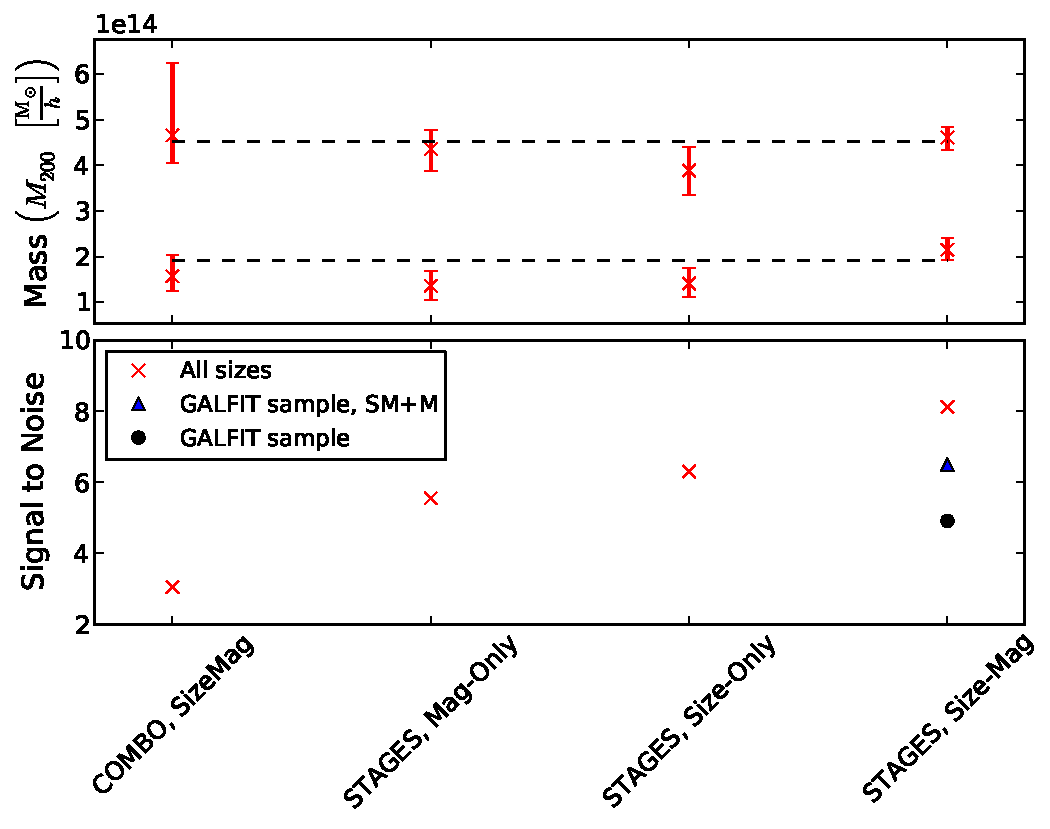
\includegraphics[width = 0.5\textwidth]{Figures/Mock_Application/Experiment_Comparison_wStN_10Run.pdf}
\caption[Example results for a size-only, magnitude-only and joint size-magnitude cluster reconstruction using mock STAGES and COMBO data, with signal--to--noise]{Comparison plot between the size-only, magnitude-only and size-magnitude analyses for both mock COMBO- and the mock STAGES-datasets for an example single run of the analysis. The {\it top} panel shows example runs for each case. In all cases, a single cluster was modelled on the field to avoid bias due to overlap between clusters, and the prior was constructed on the unlensed STAGES dataset. Errors are 68\% confidence limits of the recovered posterior about the mode position. Dashed lines show the input mass for each case. The {\it bottom} panel shows signal-to-noise, calculated as the mode point divided by half the total error width for each comparison. One can see that the size-magnitude analysis with the full STAGES set gives the largest signal-to-noise of all four cases, motivating its use on the full STAGES dataset} \label{fig:Experiment_Comparison}
\end{figure}

\begin{table}
\begin{center}
\caption{The average width of $1\sigma$ error bars taken over 10 mock realisations, for each probe considered in Figure \ref{fig:Experiment_Comparison}.}\label{Table:Experiment_Average_Noise}
\begin{tabular}{|l|c|c|}
\hline
Input: & \multicolumn{2}{c|}{$r_{200} = 1.2 h^{-1}{\rm Mpc} ;\; M_{200} \sim 20\times10^{13} h^{-1}M_{\odot} $} \\
\hline
\\
Experiment & $\bar{\sigma}_{r_{200}} [h^{-1}{\rm Mpc}]$ & $\bar{\sigma}_{M_{200}} (\times 10^{13}) [h^{-1}M_{\odot}] $ \\
\hline
COMBO Size-Mag &0.14 & 6.6 \\
\hline
STAGES Mag-Only &0.07 & 3.5 \\
\hline
STAGES Size-Only & 0.07 &  3.1\\
\hline
STAGES Size-Mag & 0.05 & 2.4\\
\hline
\end{tabular}
\end{center}
\end{table}

Figure \ref{fig:Analysis_Bias_STAGES_SizeMag} shows the fractional bias, given as
\be
f = \frac{M^{ML}_{200}-M^{\rm Input}_{200}}{M^{\rm Input}_{200}},
\ee
where $M^{\rm Input}_{200}$ is the input mass and $M^{ML}_{200}$ is the mode point of the combined posterior across 10 mock catalogue realisations. It is evident that there is no evidence for significant bias in the application of the method to the simplified case presented here. Posterior construction using the size-magnification or flux-magnification effects individually have also been verified to be similarly unbiased, but as the expected signal--to--noise is largest for the joint magnification analysis, I will focus on the use of the joint size-magnitude analysis on the full STAGES data-set for the remainder.

\begin{figure}
\centering
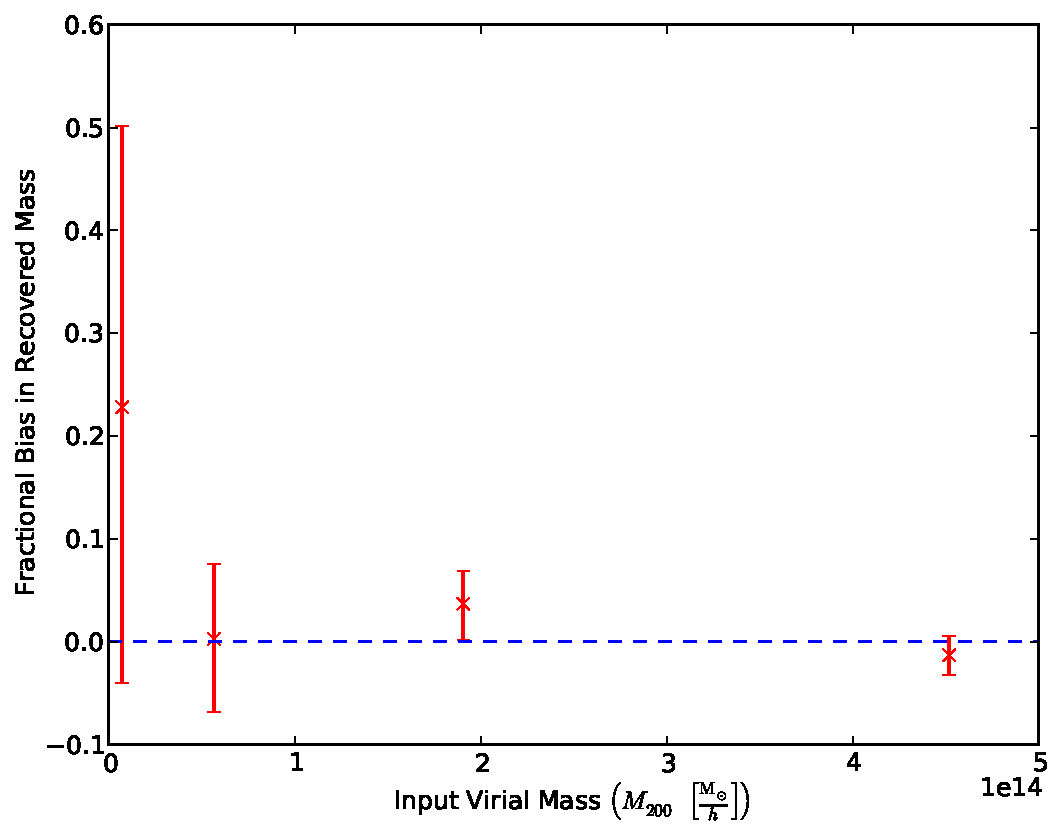
\includegraphics[width = 0.45\textwidth]{Figures/Mock_Application/SizeMag_Unbiased.pdf}
\caption{Plot showing fractional bias in cluster mass in the application of the joint size-magnification analysis on the STAGES dataset for four input cluster masses. No significant bias in recovered halo mass is evident for the ranges of masses considered here.} \label{fig:Analysis_Bias_STAGES_SizeMag}
\end{figure}

The reader is encouraged to note that the results presented here suggest that the use of the joint size and flux magnification signals can probe the large clusters of the STAGES field to high significance for the idealised case considered up to this point, however the application of the method to data presents additional problems which are so far not taken into account. As stated in Section \ref{sec:Source_Selection} the use of STAGES data complicates the removal of cluster members from the source sample due to the lack of multi-band photometry for the majority of galaxies. In part, the contamination of cluster members can be minimised by the removal of sources using a redshift cut and bright magnitude cut on the sample, however cluster contamination in the data sample remains even after the application of these cuts. As motivated in Section \ref{sec:Source_Selection}, the presence of cluster members in the source sample can be minimised by the subtraction of sources close to the core of the cluster, and such core cuts were motivated for the STAGES data considered. Whilst this application also includes redshift and magnitude cuts and a generic core cut of $0.5'$ to the source sample, stricter core cuts such as those motivated for the data will reduce the number density of the sample and result in an increase in statistical noise and subsequent reduction in signal--to--noise ratio over those presented here, where cluster contamination has been largely neglected. 

The presence of cluster member in the source sample, and non-negligible measurement error on source size may also introduce bias in the recovered posteriors. We consider the effect of such contamination on the accuracy of the method in the next two sections.

\subsubsection{Bias due to cluster member contamination}

In section \ref{sec:Source_Selection}, we noted that the presence of cluster members in the source sample can introduce a bias in the recovered cluster when not accounted for in the a-priori redshift distribution of the sources. In that section, we detailed the methods by which the source sample was selected to minimise this effect, including the application of core cuts around the main over-densities in the field, and the use of a bright magnitude cut as well as a redshift cut where the source also falls into the COMBO-17 sample. In this section, we consider the effect of cluster contamination on the recovered mass for the STAGES clusters.

Cluster contamination is modelled in the mock catalogues by constructing a cluster member catalogue according to the magnitude-only cluster contamination profile shown in Figure \ref{fig:magDiff_byMeasure}, where each annulus bin is assigned a number of cluster contaminants given by 
\be
N_{\rm Contaminant} = fn^{\rm mock}_{\rm global}\Omega - N_{\rm annulus}^{\rm Poisson},
\ee
where $f = n_{\rm annulus}/n_{\rm global}^{\rm data}$ as measured from Figure \ref{fig:magDiff_byMeasure}, $n^{\rm mock}_{\rm global}$ is the global number density of sources in the un-contaminated mock catalogue, $\Omega$ labels the area of the annulus, $N_{\rm annulus}^{\rm Poisson}$ the number of sources in that annulus in the un-contaminated mock catalogue. Where $f\le 0$, no cluster members are added to the catalogue. Thus, the cluster catalogue is constructed such that the contamination fraction of the mock is equal to that measured in the data where $f\ge 0$. The cluster members are randomly placed within the annulus, with a size and magnitude jointly randomly sampled from the reference data catalogue with $m\ge 23$ (to mimic the data cuts used in the construction of the contamination profile of Figure \ref{fig:magDiff_byMeasure}), and assigned a redshift of $z = 0.165$.  This cluster catalogue of unlensed members is concatenated with the original source catalogue after the source catalogue has been lensed by a model NFW profile. For each cluster considered, the cluster catalogue is constructed according to the measured contamination fraction profile for that cluster, given in Figure \ref{fig:magDiff_byMeasure}. Each cluster is modelled individually, and a core aperture mask of $1.2'$ around A901a, $1.2'$ around A901b, $0.5'$ around A902 and $0.9'$ around SW is applied in the application of the cluster mass measurement to mimic the application to data. %Unbiased result are therefore expected by nature, since the same core is removed as that which is used to add the contamination in the first place - this plot is therefore only informative if a comparison to one without cuts is also shown.

Figure \ref{fig:ClusterContamination_Mocks_SizeMag} shows the average signal--to--noise and fractional bias on recovered virial radius using a joint size-magnitude analysis over 10 mock realisations using the above method of mock construction. In each case, the cluster is modelled individually to avoid overlap bias, and is positioned on the measured BCG of A901a. Cluster contaminants are added in annuli up to $3'$ from the centre of the cluster. Typically, A901a contains 140 contaminants ($\sim 7\%$ of total sources within $3'$), A901b contains $\sim 300$ ($\sim 16\%$), A902  $\sim 60$ ($\sim 3\%$) and SW $\sim 80$ ($\sim 4.5\%$) when core masking is not used.  The top panel shows the fractional bias for each modelled cluster as a function of input cluster virial radius. We see that in the presence of cluster contaminants, there is no strong evidence for bias amongst all modelled clusters, with the possible exception of A901b which shows evidence of a small negative bias of a few percent, particularly at larger virial radius where the statistical noise is smallest. The bottom panel shows the average signal--to--noise on the virial radius for each cluster, where A901a and A901b are modelled as clusters with $r_{200} = 1.2 h^{-1}{\rm Mpc}$, and A902 and SW with $r_{200} = 0.8 h^{-1}{\rm Mpc}$. Errors are the variance of the mean signal--to--noise across these realisations. The control sample takes 10 realisations where the catalogues are constructed without a contamination sample; as the core masking and choice of input virial radius for A901a and A901b are identical, the control signal--to--noise for these clusters are taken to be identical. The reduction in signal--to--noise in the A902 control sample over A901a and A901b is due to the reduction in the input virial radius (and consequently viral mass) of that cluster, and the further reduction in SW is a result of the stricter core masking used in that case. We see no evidence for a significant change in the signal--to--noise in any of the clusters when cluster contamination is added: the difference between the control and cluster contamination points for A901a can be explained by a slight high bias in the control run, combined with a slight low bias in the contaminated run, both within statistical uncertainties of the input virial radius. 

\begin{figure}%htb
\centering
  \begin{tabular}{@{}c@{}}
    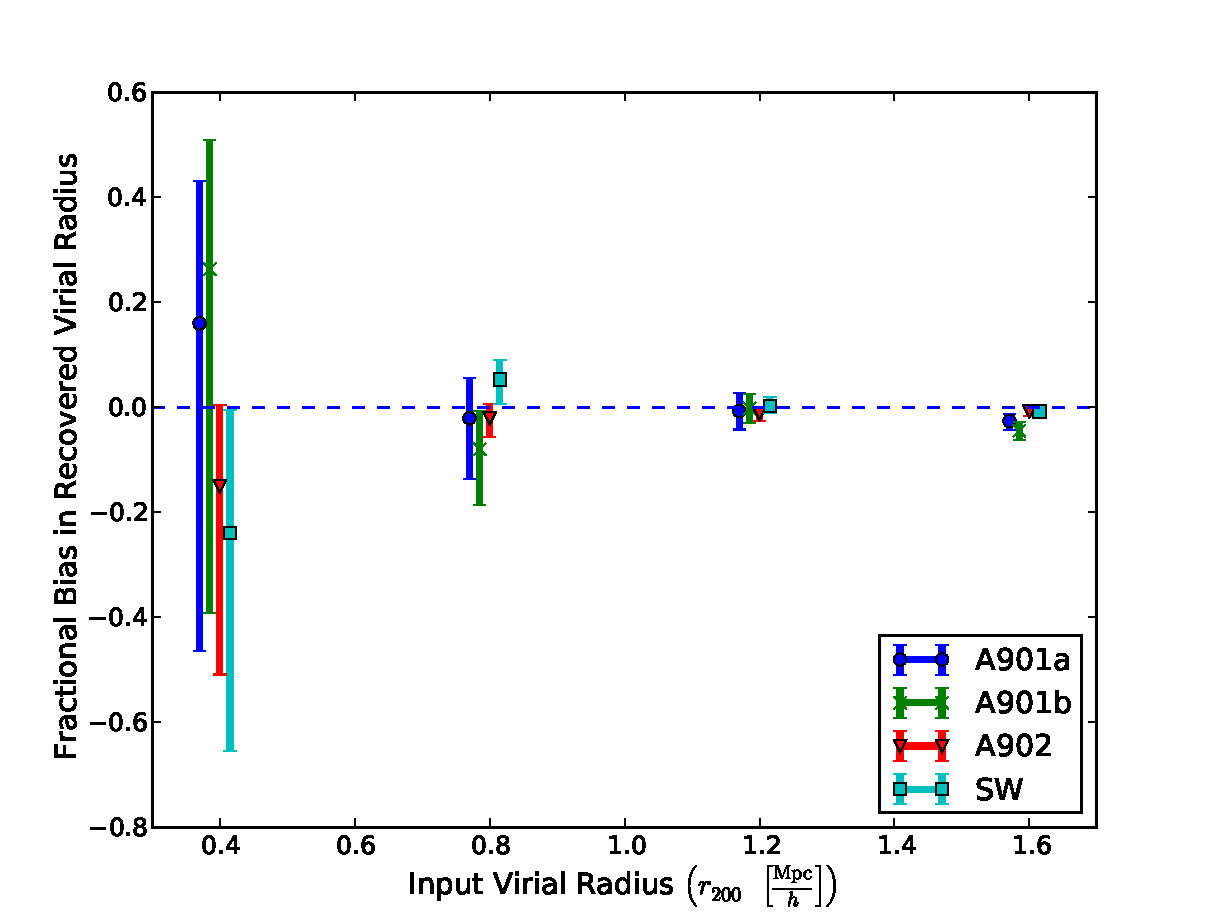
\includegraphics[width=0.45\textwidth]{Figures/Mock_Application/ClusterContamination_SizeMag_Bias_MagCutOnly.pdf} \\
    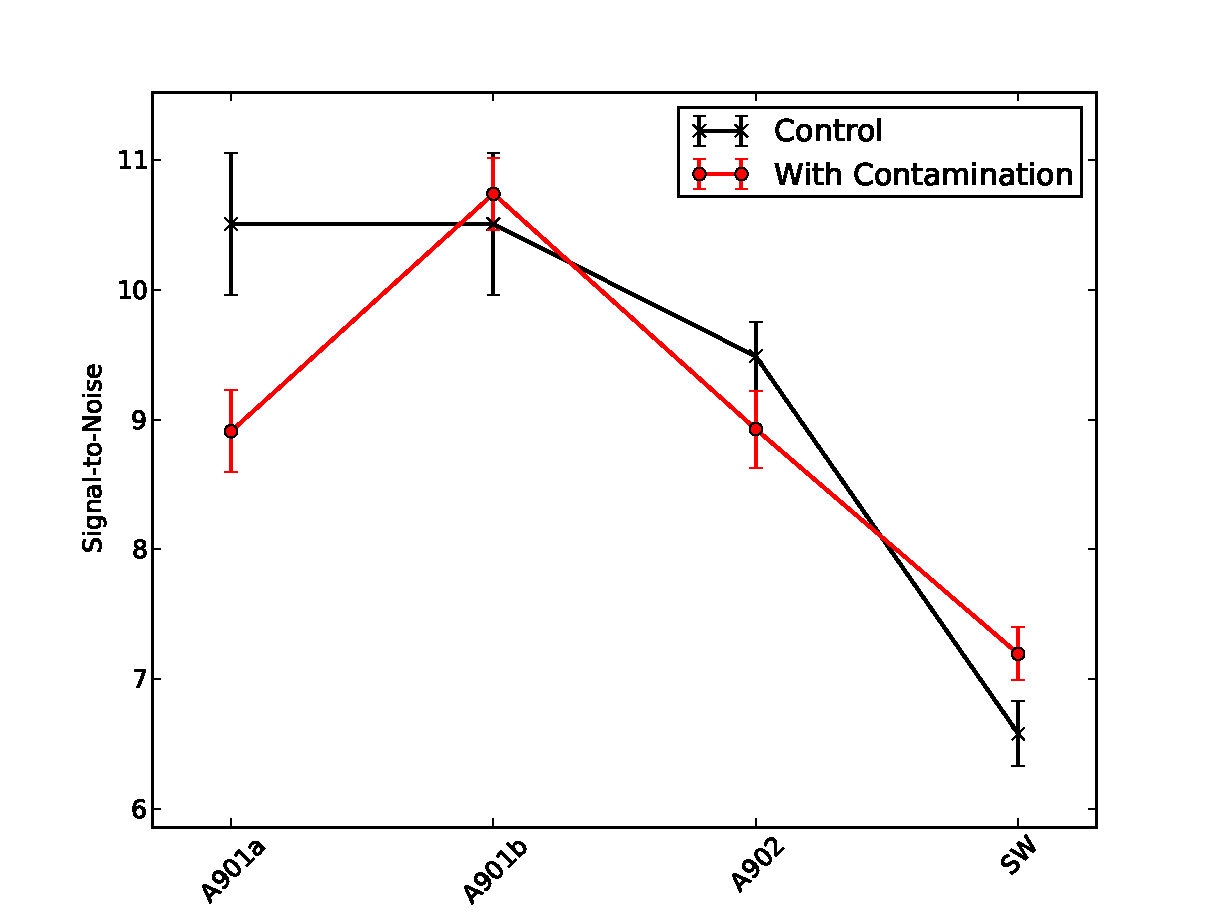
\includegraphics[width=0.48\textwidth]{Figures/Mock_Application/ClusterContamination_SizeMag_Signal-To-Noise_MagCutOnly.pdf} 
  \end{tabular}
  \caption[Fractional bias on recovered cluster virial radius due to a sample of unremoved cluster contaminants]{Figure showing the effect of a sample of cluster contaminants on the recovered posterior on the cluster virial radius. The {\it top} panel shows the fractional bias in virial radius for the contaminated catalogue as a function on modelled virial radius. Data points are slightly offset in the x-value to aid visualisation. The {\it bottom} panel shows average signal--to--noise for each cluster, where A901a and A901b are modelled using $r_{200} = 1.2 h^{-1}{\rm Mpc}$, and A902 and SW using $r_{200} = 0.8 h^{-1}{\rm Mpc}$. All values are calculated over 10 mock realisations of the catalogue, where each cluster is modelled individually to avoid overlap bias. The posterior is calculated for each cluster using the core masking for that cluster detailed in section \ref{sec:Source_Selection}, with number of contaminant clusters chosen to match the profile of Figure \ref{fig:magDiff_byMeasure} where an over-density is observed.}\label{fig:ClusterContamination_Mocks_SizeMag}
\end{figure}

Figure \ref{fig:ClusterContamination_Mocks_SizeMag} indicates that the choice of core masking aperture applied to the data is sufficient to remove any bias caused by cluster contamination of the sort considered here, with only a small bias in A901b.  However, one must note that these results consider a particular simplified form of cluster contamination, with only the inclusion of an unlensed contaminant sample, and does not account for intrinsic magnitude- or size-density correlations due to physical processes during galaxy formation. The investigation of these issues are left for future work.

%%Note that this does not consider intrinsic size-density correlations 

\subsubsection{Bias due to measurement noise}\label{sec:NoiseBias}

In Section \ref{sec:Reconstruction_Method}, we noted that the pipeline as detailed does not explicitly account for measurement error on measured source size and briefly detailed how one may edit the likelihood evaluation to account for measurement noise in any of the observed quantities. In this section, I quantify the expected bias due to unaccounted-for error in the measured size and magnitude in the idealised STAGES catalogue.

In the method of mock catalogue construction detailed in Section \ref{sec:Mock_Catalogue_Construction}, it is assumed that the measured sizes are exact, and that any variation in measured size is due only to lensing by foreground structure. Measurement noise is included int the mock catalogue construction by adding an uncertainty sampled from a Gaussian distribution with width $\sigma_T = 0.2T$ and $\sigma_m = 0.08$, after sizes and magnitudes have been sampled from the master catalogue and before lensing by the simulated cluster. This approximately corresponds to the measured uncertainty in PSF-corrected quadrupole sizes for the high signal--to--noise sources considered in Appendix \ref{sec:STAGES_RRG_Measurement}, and the average measured uncertainty in the GALFIT scale radius in bins of measured scale radius, taken directly from the master catalogue, and the magnitude uncertainty is taken to be the mean MAG\_BEST uncertainty across the entire field. The measurement noise therefore is included in the unlensed catalogue, which is used to construct the a-priori size distributions for the application to mocks, as well as the source sample in the measurement with the pipeline. 

Figure \ref{fig:Measurement_Noise_Bias_SM} shows the fractional bias in recovered mass over ten mock realisations, for four input cluster masses. We see that there is evidence for a negative bias in the recovered mass, whose absolute value decreases with increasing cluster mass, corresponding to the decreasing bias with increasing signal--to--noise. Thus, we expect that the recovered cluster masses in the application of this method with be biased low, with the smallest clusters most affected: in practice, this would suggest that the measurement of cluster mass for A902 and the SW group should be more affected by noise bias than the larger A901a and A901b clusters, with a predicted $\sim 20\%$ and $\sim 10\%$ bias for both sets respectively. This bias is comparable to the expected uncertainty on the recovered mass for each of these clusters, and thus represents the largest potential impact to recovered cluster mass of any of the potential sources of bias we have considered in this analysis

In practice, one may take the uncertainty on the measured size and magnitude into account naturally using the method presented in Section \ref{sec:Reconstruction_Method} by marginalising over a latent variable which describes the distribution of the measured size or magnitude around the true underlying value. In doing so, one naturally increases the computational run-time which is already limited by the need to marginalise over a redshift distribution for each sources in the source sample for each evaluation of the cluster profile parameters. For a large source sample, such as that considered here and required by the desire to simultaneously fit all clusters in the field, this additional run-time can become computationally expensive, and so we note this bias an leave the application with the inclusion of measurement noise to future work. 

\begin{figure}
\centering
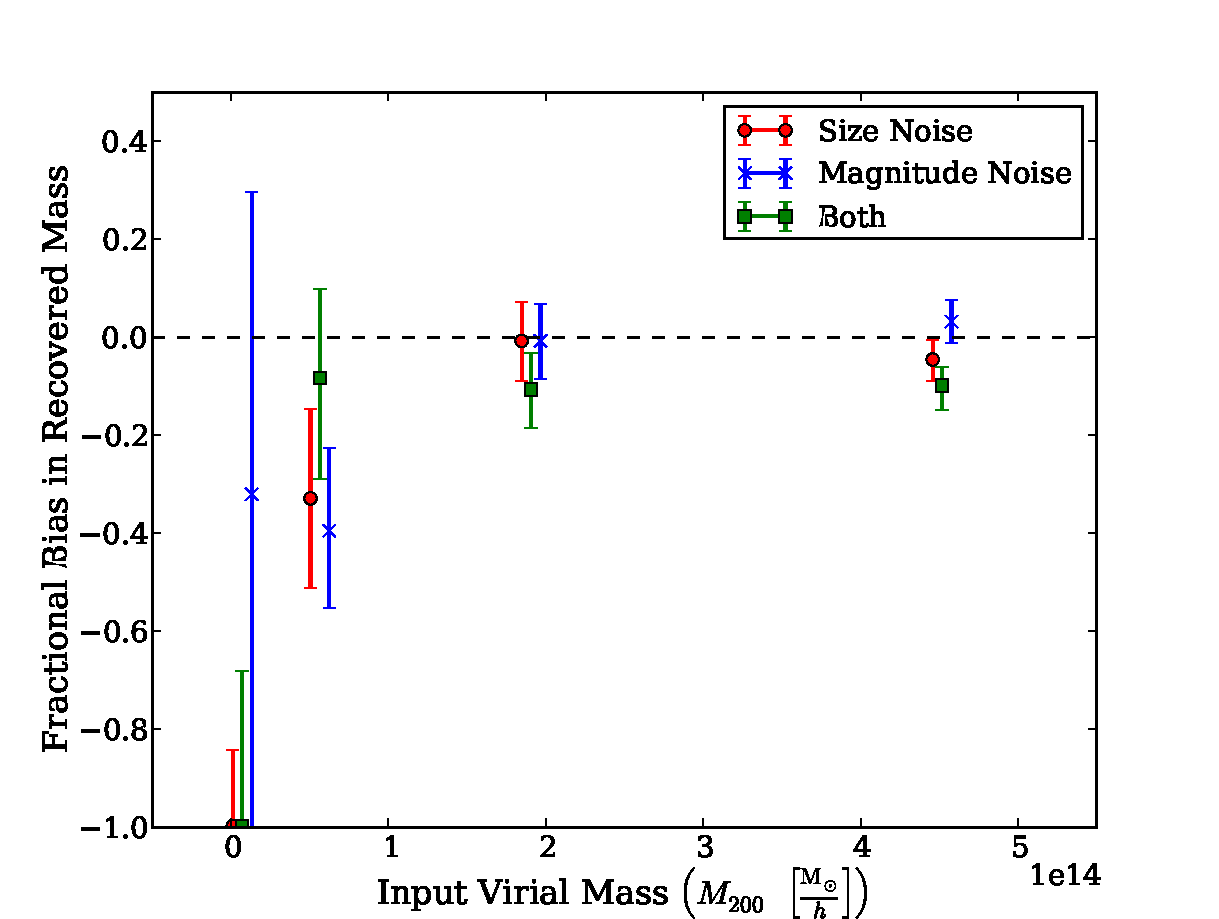
\includegraphics[width = 0.5\textwidth]{Figures/Mock_Application/NoiseBias_Size_Mag_Both.pdf}
\caption{Plot detailing the bias in recovered mass from a joint size-magnitude analysis resulting from noise in the size and magnitude measurements, when this is not taken into account in the analysis. Red circles correspond to the application of Gaussian noise on size with mean zero and  $\sigma_T = 0.2T$, blue crosses a constant Gaussian noise on magnitude with with $\sigma_m = 0.08$, and green squares the combination of both. Ordinate values are offset for ease of visualisation, , and each group of three corresponds to simulated NFW clusters with virial radii of $r_{200} = 0.4,0.8,1.2,1.6$ $h^{-1}$Mpc respectively.}\label{fig:Measurement_Noise_Bias_SM}
\end{figure}

\section{Application to STAGES}\label{sec:ApplicationToSTAGES}

In the previous section, we have shown that the application of the proposed method of cluster model parameter determination detailed in Section \ref{sec:Reconstruction_Method} provides a means to accurately measure the mass of mock clusters with a STAGES-like data-set, and quantified any biases resulting from simplifications in the pipeline, or limitations in the data. In this section, we apply the method to the STAGES data-sets detailed in section \ref{sec:Source_Selection}, and quantify cluster model parameter constraints for the STAGES clusters, with a comparison to existing measurements using source shape in \cite{Heymans:2008p2060}. Following \cite{Heymans:2008p2060}, we consider a fit using four clusters (A901a, A901b, A902 and SW), and a 6-cluster fit (where A902 and the SW group are split into two component clusters, A902, CB1, and SWa and SWb respectively).

\subsection{Mass Reconstruction of the STAGES clusters}

Unless otherwise stated, the cluster virial radius are allowed to vary independently for considered clusters. The cluster redshift is enforced to be $z =0.165$ for all clusters with the exception of CB1, which is placed at $z = 0.46$ in accordance with the results of \cite{Taylor:2004p2808}. The mass-concentration relation is set using the fit of \cite{Dolag:2004p2721}. The application of this relation follows the results of \cite{Heymans:2008p2060}, and therefore allows a more direct comparison between both sets of results, however we note that the concentration may be simultaneously fit along with the other cluster model free parameters, and the consideration of this case is left to future work. Constraints are produced using a Markov-Chain-Monte-Carlo method, and convergence of the recovered posteriors is enforced by requiring that the marginalised posteriors for each free parameter satisfy $R<1.03$, where $R$ is the Gelman-Rubin statistic.

Figure \ref{fig:MassRecon_BCG_4Cluster} shows the result where four over-densities are fit across the field on the BCGs of the main over-densities. Diagonal panels show the one-dimensional marginalised posteriors for each single model parameter for each cluster, whilst off-diagonal panels show the two-dimensional marginalised posteriors between two model parameters, with all other parameters across all clusters marginalised over. Vertical lines show the quoted mean (solid) and 1-$\sigma$ uncertainty for the shear analysis of \cite{Heymans:2008p2060}. We immediately see that the magnification measurement detects all four clusters, with a signal--to--noise--ratio on the virial radius of $9.3,5.35,3.47,5.11$ respectively. 

\begin{figure*}
\centering
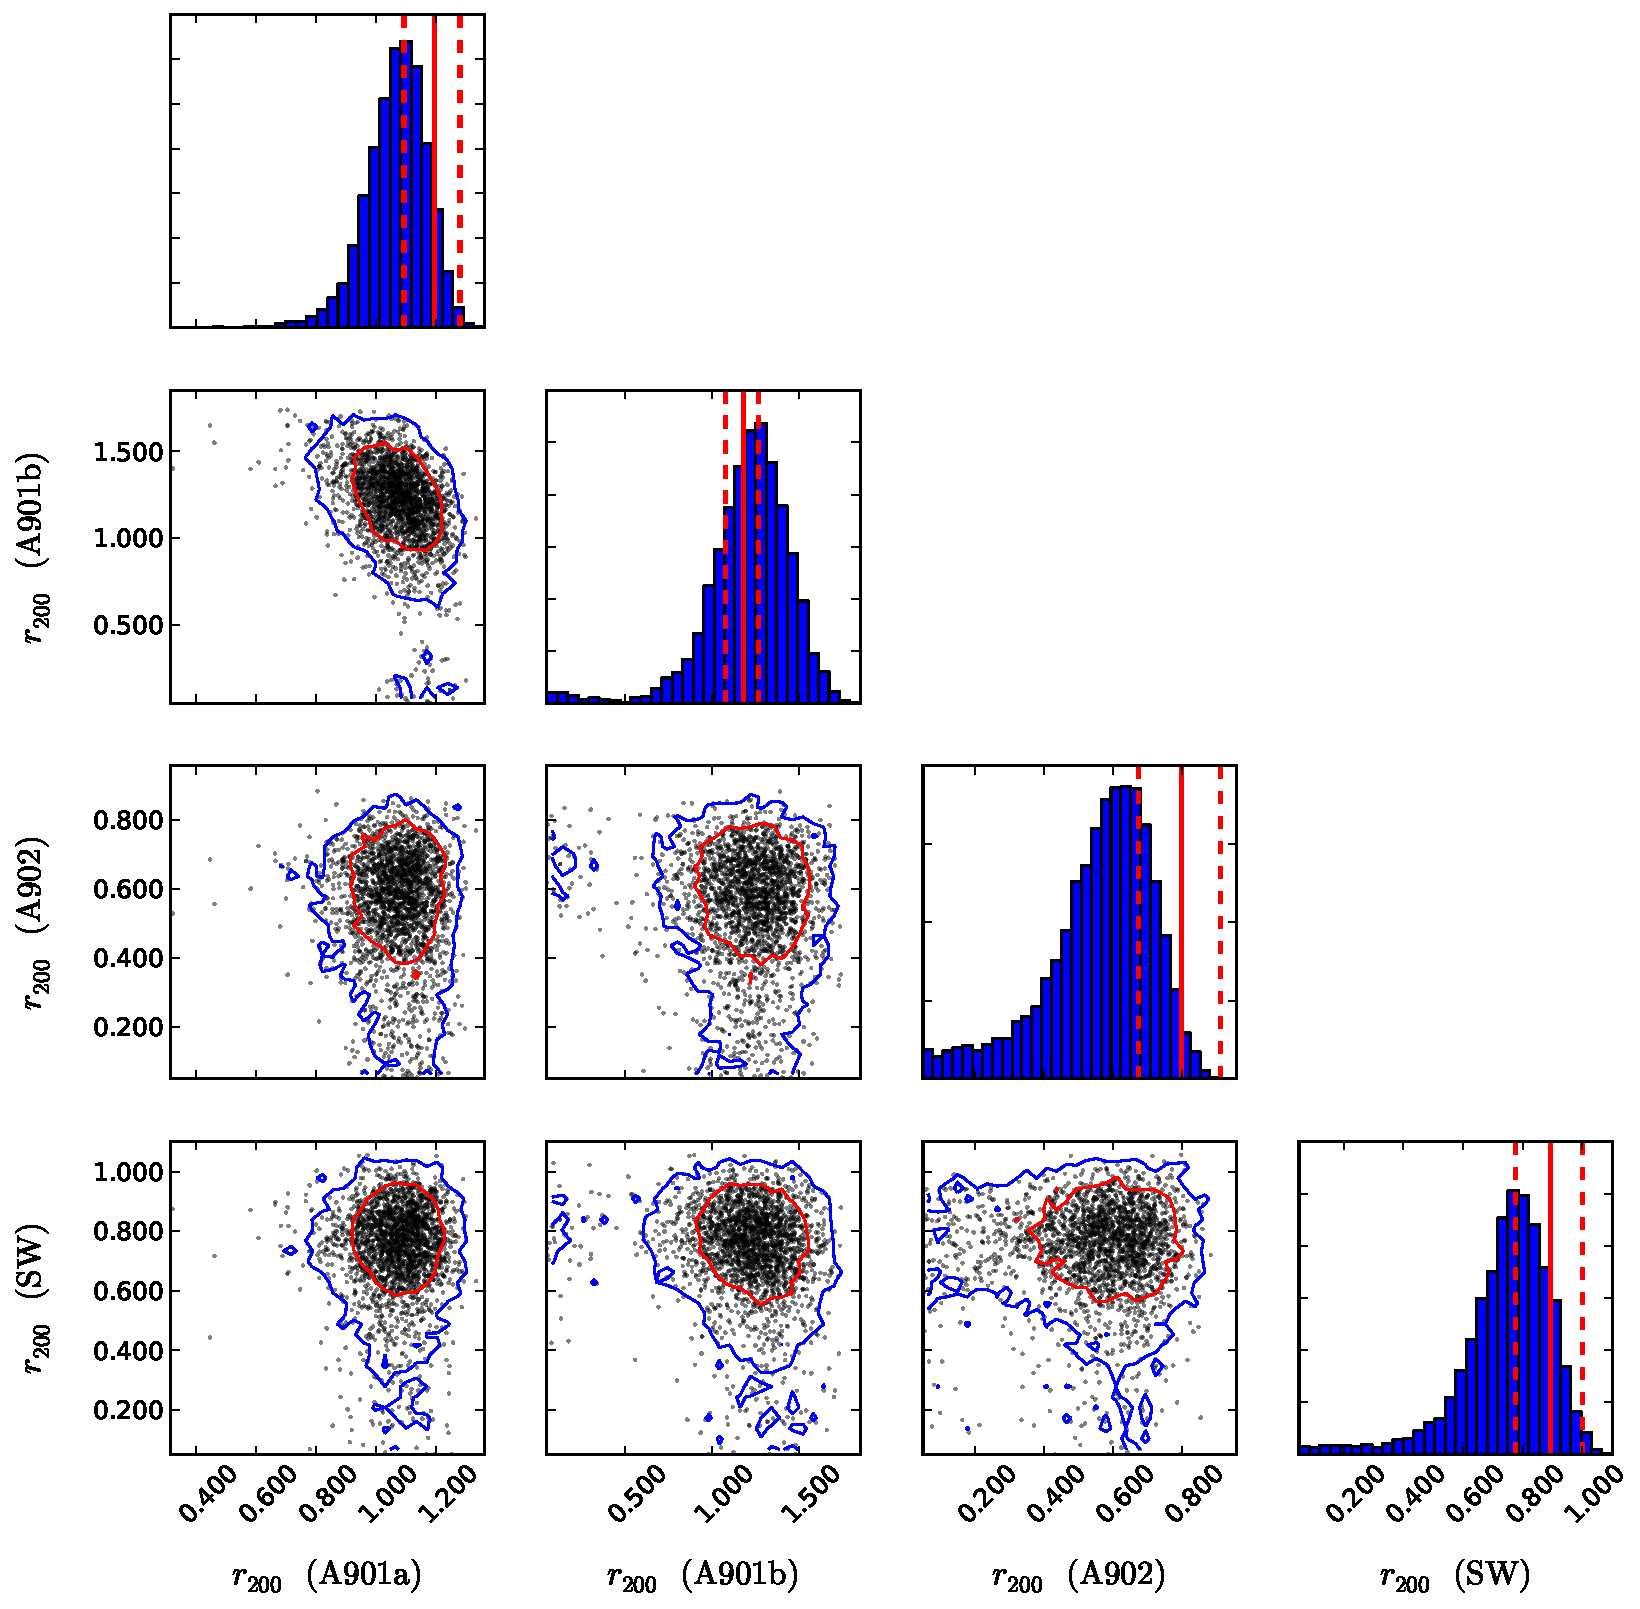
\includegraphics[width = 0.95\textwidth]{Figures/Data/Mass_Reconstruction/MCMC_DistributionPlot_4Cluster_BCG_MassOnly.pdf}
\caption{Result of the application of the method in the case where 4 clusters are considered (A901a,A901b, A902, SW) centered on their BCGs. Diagonal plots show the marginalised distribution for the virial radius on each cluster, and the vertical red lines show the mean (solid) and 1-$\sigma$ uncertainty (dashed) for the shear analysis given in \cite{Heymans:2008p2060}. Off diagonal plots show points from a thinned MCMC chain, and black, blue and red lines show the 68-, 95-, and 99\% confidence regions for the 2D marginalised distributions respectively.} \label{fig:MassRecon_BCG_4Cluster}
\end{figure*}

\begin{figure*}
\centering
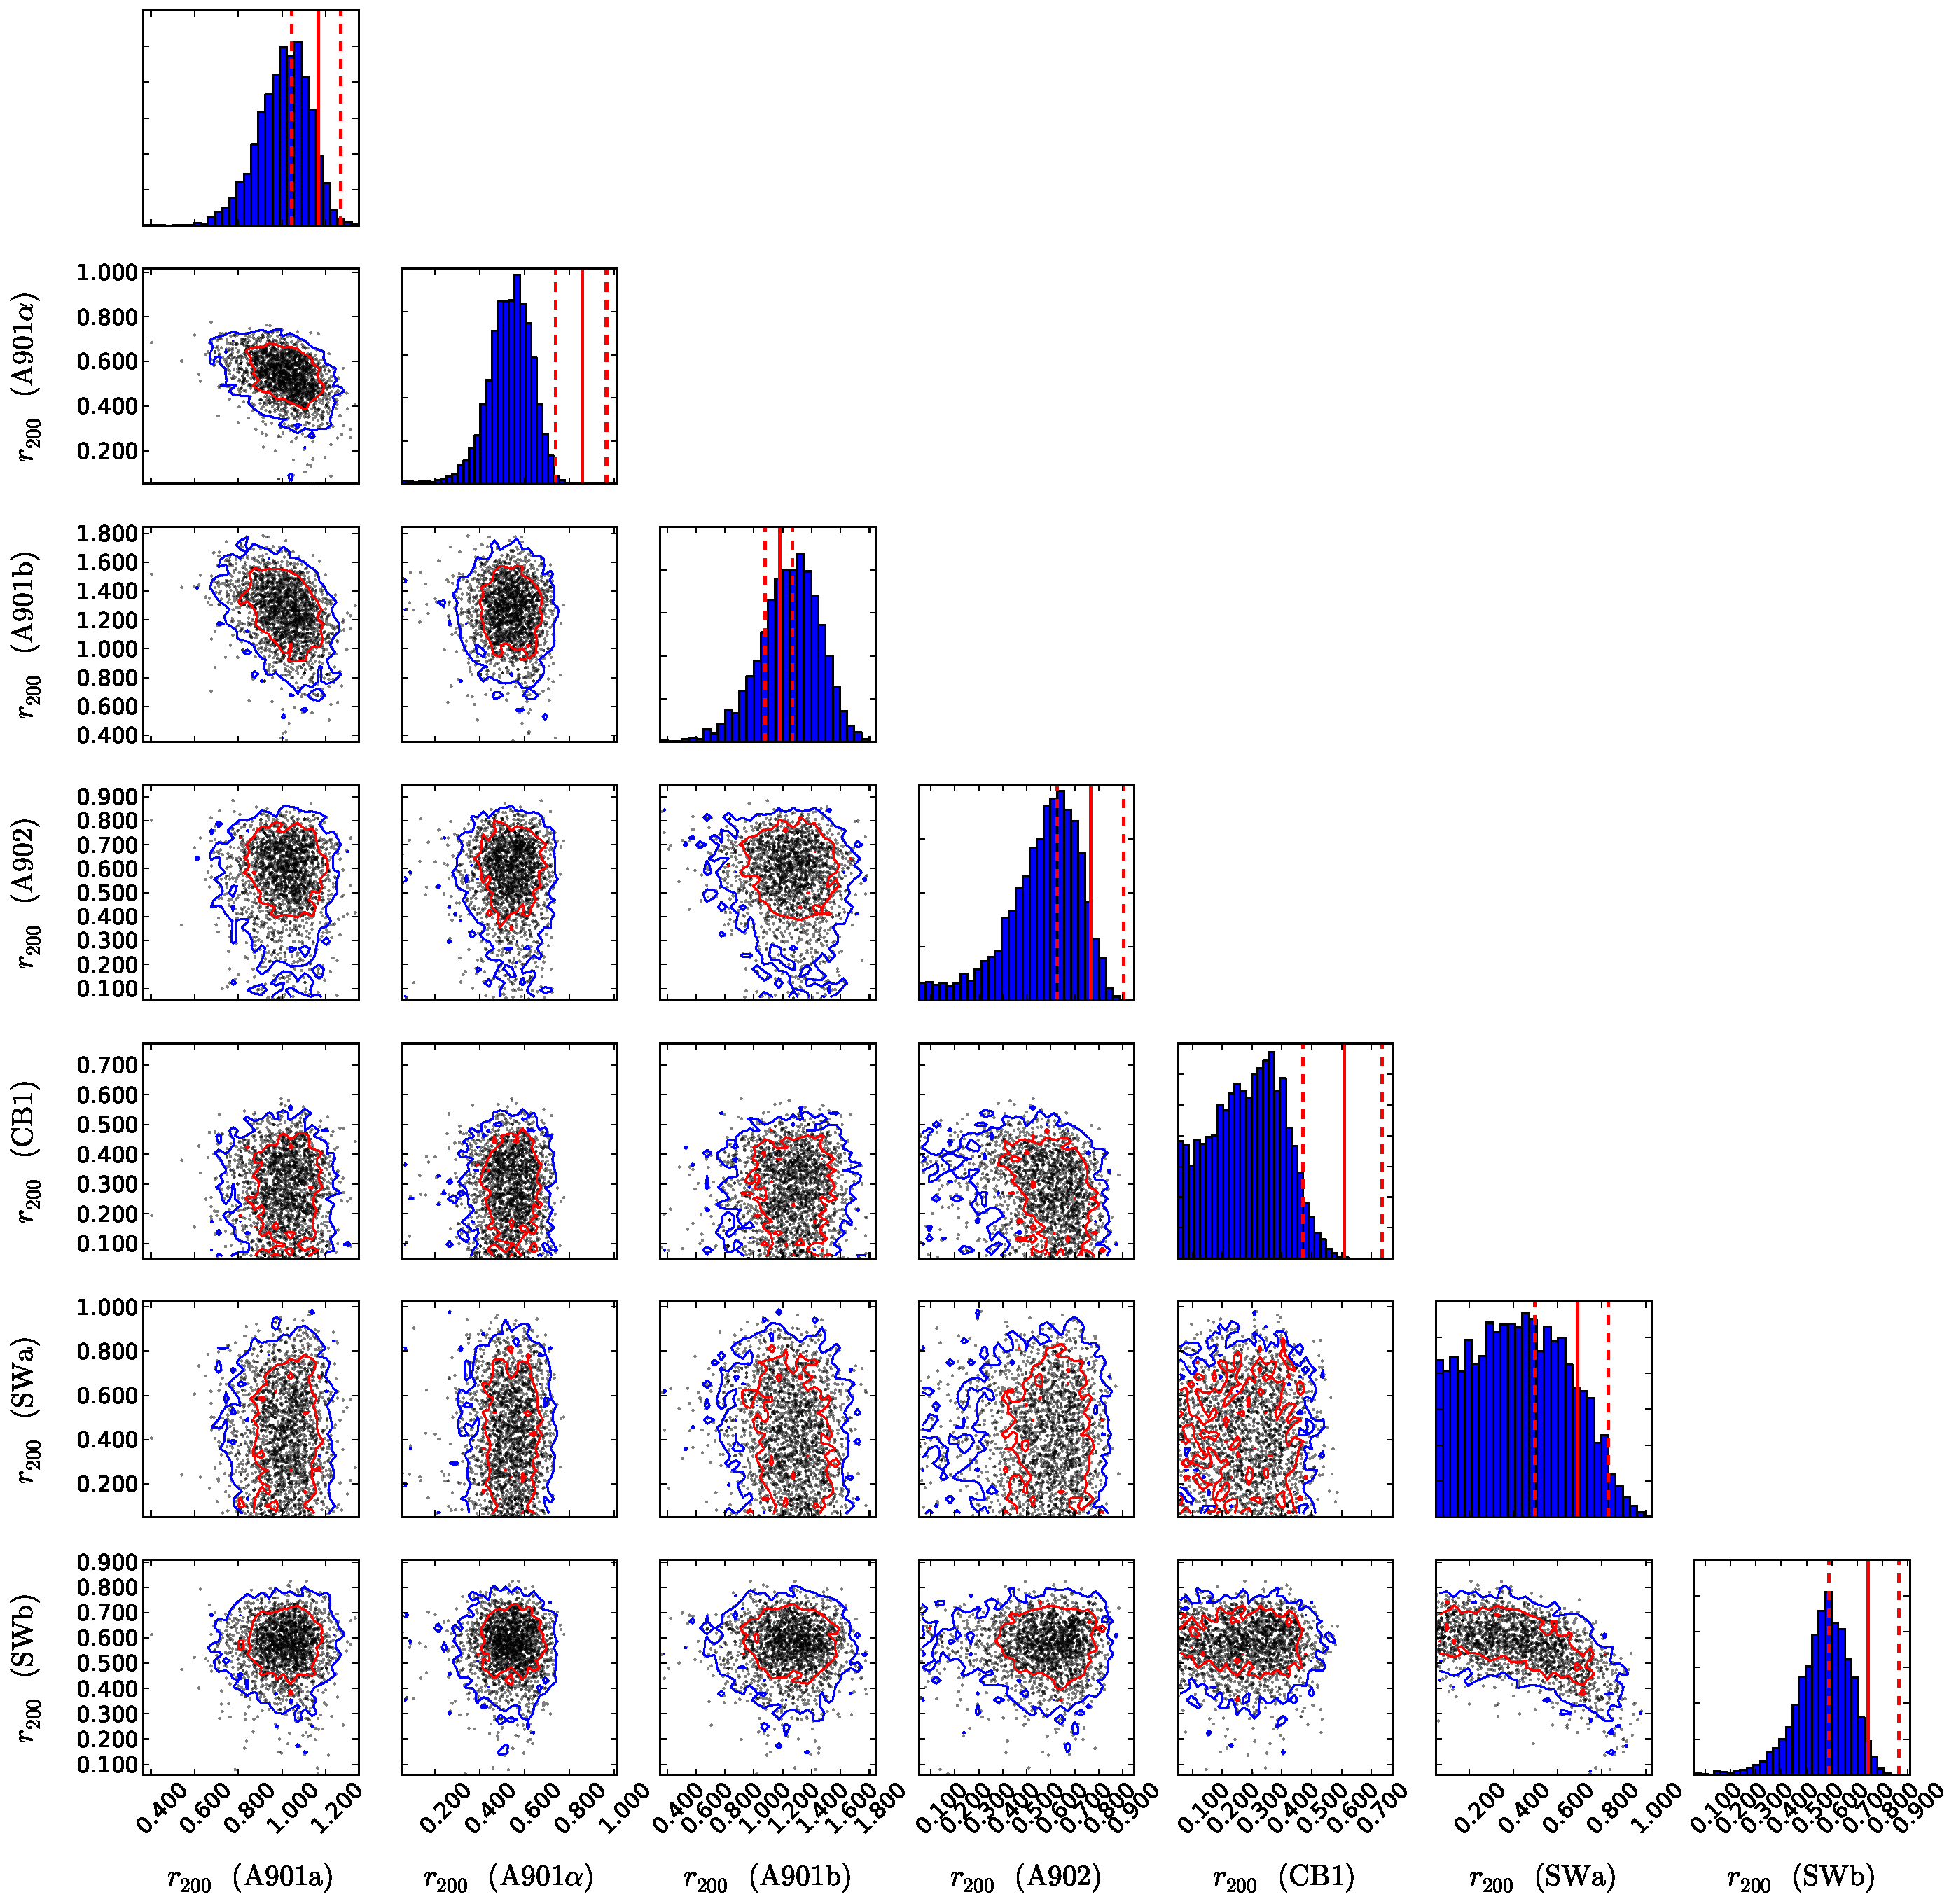
\includegraphics[width = 0.95\textwidth]{Figures/Data/Mass_Reconstruction/MCMC_DistributionPlot_7Cluster_BCG_MassOnly.pdf}
\caption{Result of the application of the method in the `two halo' case where 7 clusters are considered (A901a, A901$\alpha$, A901b,  A902, CB1, SWa, SWb) centered on their BCGs. Diagonal plots show the marginalised distribution for the virial radius on each cluster, and the vertical red lines show the mean (solid) and 1-$\sigma$ uncertainty (dashed) for the shear analysis given in \cite{Heymans:2008p2060}. Off diagonal plots show points from a thinned MCMC chain, and black, blue and red lines show the 68-, 95-, and 99$\%$ confidence regions for the 2D marginalised distributions respectively.} \label{fig:MassRecon_BCG_7Cluster}
\end{figure*}

Figure \ref{fig:MassRecon_BCG_7Cluster} shows the result in the `two halo' case, where A901a, A902 and the SW group are split into two seperate halos respectively, motivated by the shear mass reconstruction and x-ray emission (see \cite{Heymans:2008p2060} for discussion). In this case, the seven clusters are detected to a signal--to--noise of $7.27, 5.13, 5.40, 3.45, 5.33$ in virial radius for A901a, A901$\alpha$, A901b, A902 and SWb respectively. CB1 and SWb show a maximum-posterior point which is consistent with the presence of a cluster, but to much reduced significance.

These results are summarised in Table \ref{tab:NFW_res}, including mass estimates for each cluster considered. In contrast to the application to the mock catalogues which assumed a flat prior on virial radius in all cases considered, mass estimates here are presented assuming a flat prior on the mass. As a flat prior on the virial radius corresponds to a prior on the mass which diverges as the recovered mass tends to zero (see equation \ref{eqn:Mass_Radius_Prior_equiv}), where the recovered posterior does not tend to zero faster than $M^\frac{2}{3}$ the data is not strong enough to overcome the prior and giving prior-dominated posteriors peaking at $M=0$. We see that this is the case for A902 and SW in the `one halo' case, and A902, CB1 and SWa in the `two halo' case, and note that improved data may avoid this issue in future applications. However, the application of a flat prior on mass in this case also allows the easy relation between these results and those of \cite{Heymans:2008p2060}.

\begin{table*}
\begin{center}
\begin{tabular}{l|l|c|c|c|r}
\hline
Structure & RA & Dec & $M_{200}$ & $r_{200}$ & SNR\\
& (deg) & (deg)& $({\rm h}^{-1} 10^{13} {\rm M}_{\odot})$ & $({\rm h}^{-1} {\rm Mpc})$ & ($r_{200}/\sigma_{r_{200}}$)\\
\hline
One Halo\\
A901a & 149.1099 & -9.9561 & $14.95^{+3.12}_{-4.32}$ & $1.107^{+0.072}_{-0.119}$ & 9.30 \\[5pt]
A901b & 148.9889 & -9.9841 &  $21.96^{+11.34}_{-10.15}$  & $1.258^{+0.187}_{-0.235}$ & 5.35 \\[5pt]
A902 & 149.1424 & -10.1666 & $2.78^{+1.45}_{-1.78}$ & $0.631^{+0.095}_{-0.182}$ & 3.47\\[5pt]
SW & 148.9101 & -10.1719 & $5.27^{+2.50}_{-2.52}$  & $0.782^{+0.108}_{-0.153}$ &  5.11\\[5pt]
\\
Two Halo\\
A901a &  149.1099 &  -9.9561 &$13.03_{- 4.67}^{+ 3.30}$ & $1.057_{-0.145}^{+0.083}$ & 7.27 \\[5pt]
A901$\alpha$ & 149.0943 &  -9.9208 & $2.02_{- 0.97}^{+ 0.88}$ & $0.568_{-0.111}^{+0.073}$ & 5.13 \\[5pt]
A901b & 148.9889 & -9.9841 & $24.47_{- 11.23}^{+ 11.08}$  & $1.304_{-0.241}^{+0.173}$ & 5.40 \\[5pt]
A902 & 149.1424 & -10.1666 &$ 2.67_{- 1.71}^{+1.55}$ &$0.623_{-0.180}^{+0.103}$ & 3.45\\[5pt]
CB1 & 149.1650 & -10.1728 & $0.46_{- 0.40}^{+ 0.44}$ &$0.346_{-0.172}^{+0.087}$ &  2.00\\[5pt]
SWa & 148.9240 & -10.1616 & $0.93_{- 0.84}^{+2.51}$ &$0.438_{-0.239}^{+0.240}$ & 1.83\\[5pt]
SWb & 148.9070 & -10.1637 & $2.17_{-1.01}^{+1.15}$ &$0.581_{-0.109}^{+0.089}$ & 5.33\\[5pt]
%\input{NFW_res.tab}
\hline
\end{tabular}
\end{center}
\caption{Measurements of the virial radius and virial mass of the STAGES clusters, taken to be the mode and 1-$\sigma$ uncertainty on either side of the mode taken from the marginalised posterior distributions on $r_{200}$ for each cluster. RA and Dec label the centroid of each cluster considered, and are taken directly from \cite{Heymans:2008p2060}. The ``one halo'' and ``two halo'' cases are chosen to mimic the analysis of \cite{Heymans:2008p2060}, and to allow for easier comparison between masses derived using shear and magnification measurements, and centroid positions are taken from that analysis. For both the virial radius and virial mass, a flat prior on each is considered.}
\label{tab:NFW_res}
\end{table*}

%% Discussion

%%Comment on consistency with shear, competitiveness. Note expected complementarity. Note conclusions on Schmidt analysis, Heymans analysis (centroid variation?), Alsing analysis

Figure \ref{fig:MassRecon_BCG_4Cluster} shows the comparison between the maximum-posterior estimate of the cluster virial radius from the shear analysis of \cite{Heymans:2008p2060} against the maximum-posterior results presented here. The top panel shows the recovered virial radius and $68\%$ confidence limit for each cluster, whilst the bottom panel shows the ratio of the total width of the 68\% confidence region in the magnification analysis to the shear analysis. We see good agreement between the magnification and shear results, however there is evidence for a low bias in the recovered virial radius, particularly for A902 and the SW group, which represent the smallest modelled over-densities on the field in this case. This is in agreement with the predictions on noise bias in section \ref{sec:NoiseBias}, and therefore it is possible that bias in the magnification estimates is a result of neglecting measurement noise in the analysis considered. We note that this low bias in the magnification analysis is in agreement with \cite{Ford:2014p2825}, who also find a low bias in the magnification results compared to shear for stacked mass reconstruction with CFHTLenS.

We see also that for A901a, A902 and SW the magnification estimate is produced with a comparable statistical uncertainty to the shear signal, with the magnification analysis producing estimates with a purely statistical uncertainty less than $20\%$ larger than the shear analysis in all three cases. This result is promising, particularly as one recalls due to limitations in the data we have applied core removal on all four clusters to reduce contamination by cluster members, thus reducing the source sample over that used for the shear analysis. Further, we do not have size measurements for the whole source sample. For A901b, the error on the magnification analysis is approximately twice as large as the equivalent-mass A901a, consistent with the reduction of the source sample around A901b through the application of a more strict faint magnitude cut (see section \ref{sec:Source_Selection}).

\begin{figure}
\centering
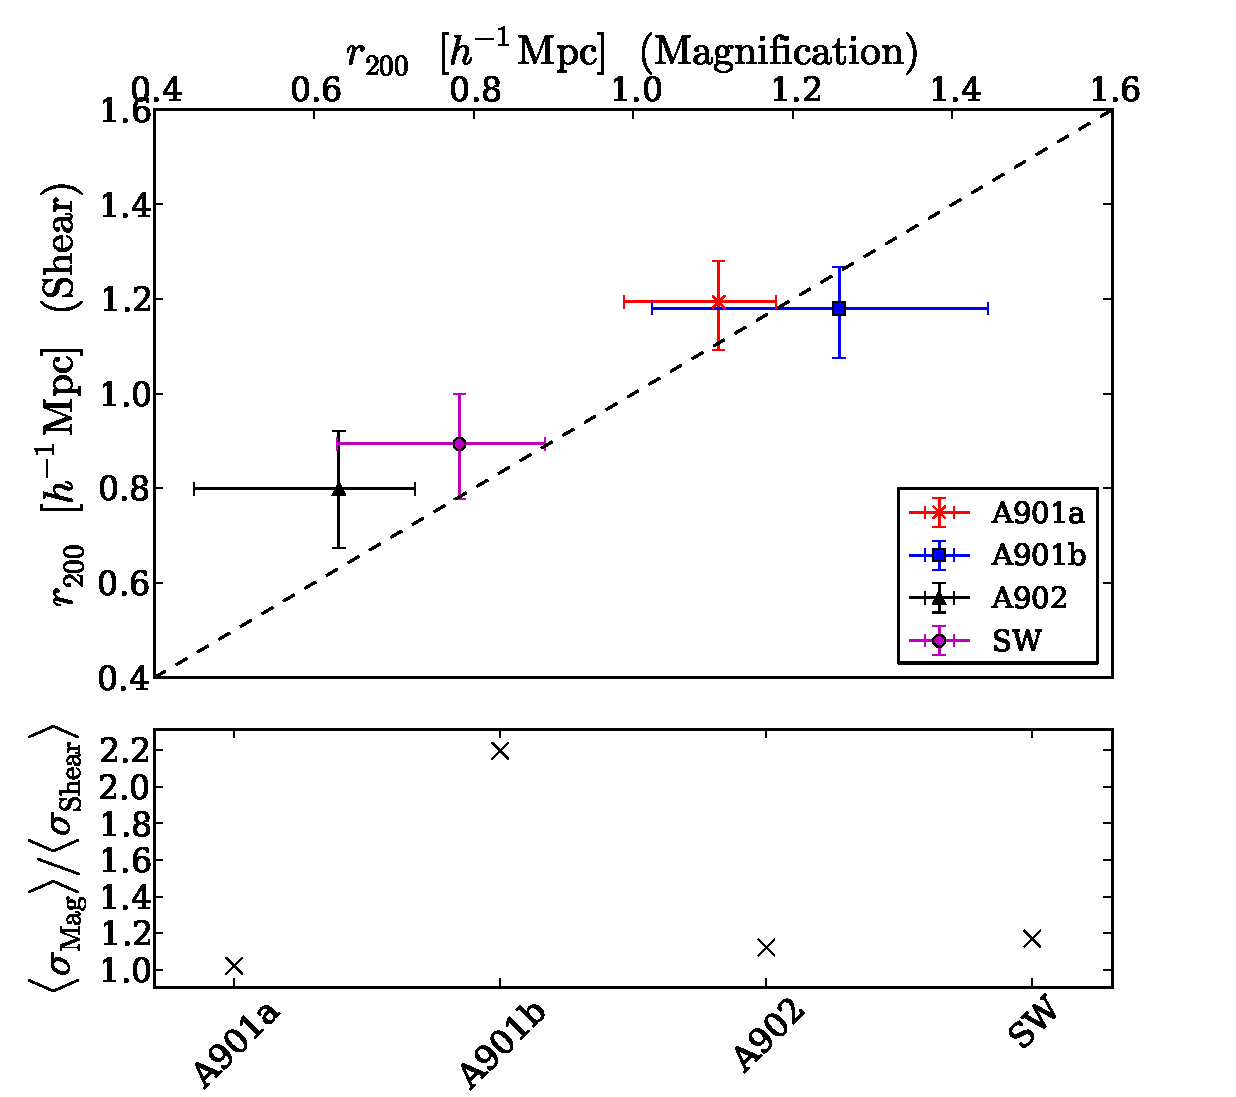
\includegraphics[width = 0.48\textwidth]{Figures/Data/Mass_Reconstruction/Shear_Mag_Comparison_4Cluster.pdf}
\caption{Plot comparing the maximum-posterior estimates and uncertainties between the described size-magnitude magnification analysis and the shear analysis of \cite{Heymans:2008p2060}, in terms of the recovered virial radius, for the one-halo case where the four main clusters (A901a, A901b, A902 and SW) are modelled on the field. {\it Top} shows the shear results on the ordinate axis, with the results of this investigation on the co-ordinate axis. The dashed diagonal line shows a one-to-one correspondence. {\it Bottom} shows the ratio of half the total 68\% confidence level with for the magnification analysis to the shear result for each cluster.} \label{fig:Shear_Mag_Comp_4Cluster}
\end{figure}

\begin{figure}
\centering
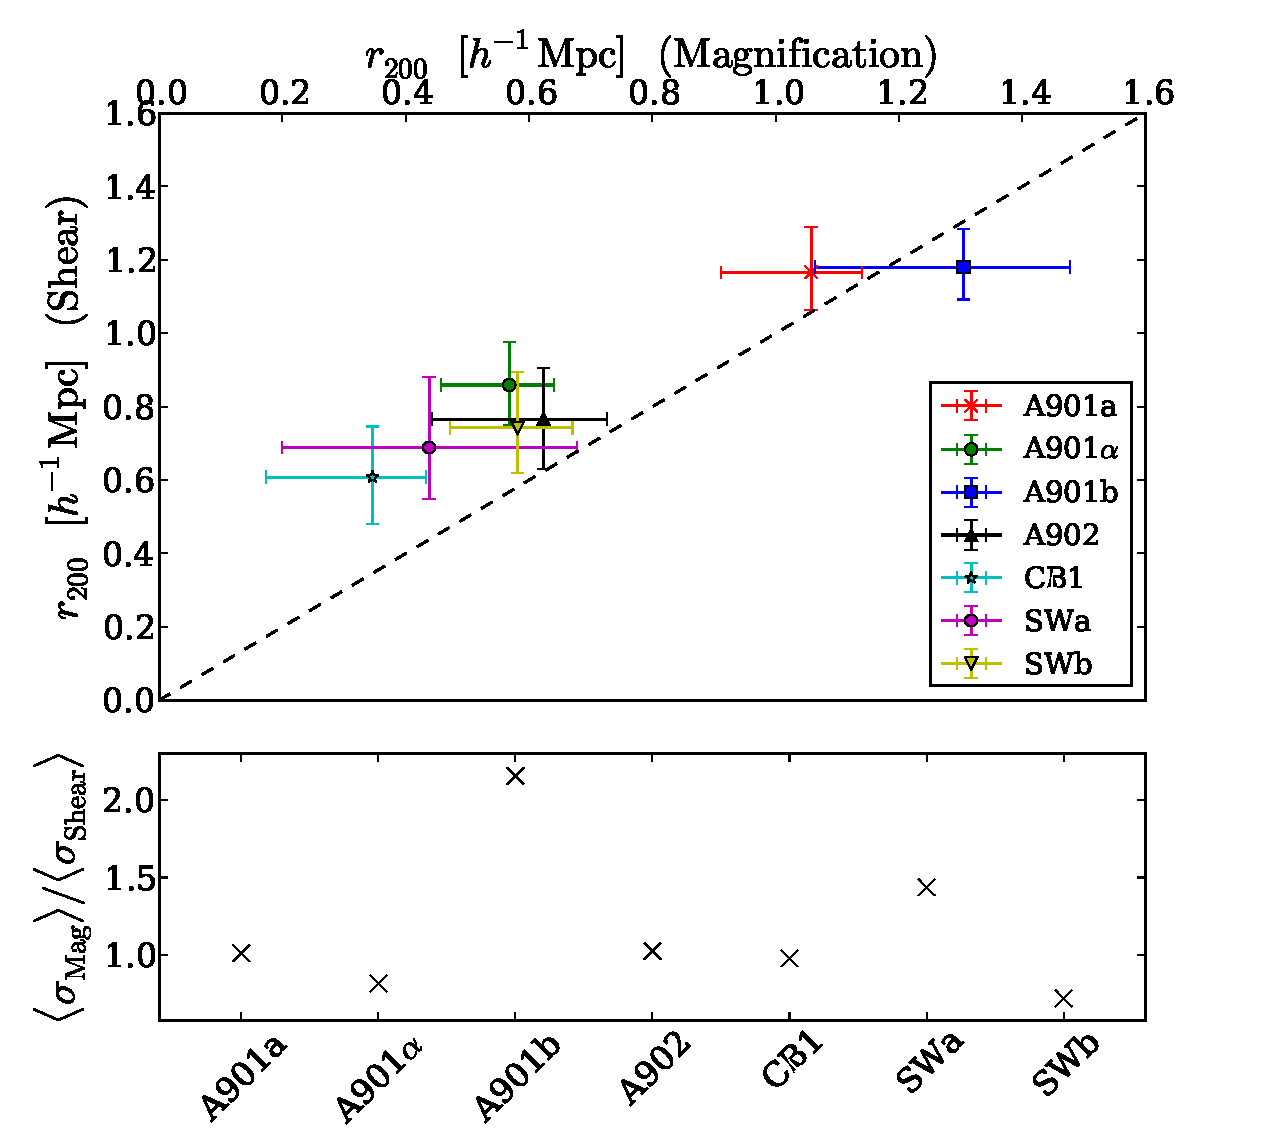
\includegraphics[width = 0.48\textwidth]{Figures/Data/Mass_Reconstruction/Shear_Mag_Comparison_7Cluster.pdf}
\caption{As Figure \ref{fig:Shear_Mag_Comp_4Cluster}, but in the `Two Halo' case.} \label{fig:Shear_Mag_Comp_7Cluster}
\end{figure}

Figure \ref{fig:Shear_Mag_Comp_7Cluster} shows the same for the `two halo' case where 7 clusters in total are modelled on the field. We see similar trends to the 4 cluster case, with a low bias in the recovered virial radius from the magnification analysis when compared to the shear results. For all clusters considered, the error on the virial radius estimate from the magnification is comparable to that of the shear, with the exception of A901b resulting from the stricter cuts used around this cluster.

In comparing the results presented here, one must be aware of a few effects which can complicate such a comparison. Firstly, as explained above, in this analysis we have applied core subtraction on the source sample, which was not applied in the shear analysis. This can have multiple effects on the final result: Firstly, as well as cluster member contamination such a subtraction should make the magnification analysis less susceptible to contamination of the signal by intrinsic size- and magnitude-density correlations by removing sources close to the cluster, however equivalent intrinsic ellipticity-density correlations may be present in the shear analysis. Secondly, in both analyses it is assumed that the underlying dark matter mass profile is well described by an NFW profile with a fixed mass-concentration relation. If this is not true, then the subtraction of the core sample may introduce a discrepancy between the results through a model bias as the shear analysis is more sensitive to the core of the true lensing mass distribution than the core-subtracted magnification analysis. Thirdly, in both cases the mass profile centre has been fixed to the values used in the shear analysis, which may introduce a centroid bias which will be more significant in the directional spin-2 shear analysis than the scalar magnification field \citep[][for a description on how mis-centering may affect each measurement]{2007arXiv0709.1159J}.

As noted above, in \cite{Ford:2014p2825} an analysis of stacked 3D-Matched Filter clusters in the CFHTLenS field using magnification bias (where the number density contrast of a distinct background source sample forms the estimator for the magnification field) and shear found that the magnification-derived cluster masses where systematically lower as a function of richness, similar to the trend we find here. In that analysis, the authors also find that the recovered mass of the magnification analysis is larger than the shear in the redshift range of the STAGES clusters, in contrast to the trend seen here, however it is noted that in that range their analysis may be affected by low-redshift contamination of the Lyman-break source sample.  The authors note that varying depth and seeing across the field may also introduce systematic bias in the magnification bias signal, and we note that this may also enter this analysis if this affects the size and magnitude determination in a spatially varying way.

In \cite{Schmidt:2012p1106}, the authors presented a joint magnitude and size analysis on stacked groups in the COSMOS field, and found that the projected surface mass density from the magnification analysis was consistent with a shear analysis within the uncertainties, but with a signal--to--noise approximately $40\%$ of the shear value. In this analysis, we also find that the magnification analysis returns the cluster mass to a lower signal--to--noise, however the reduction here less severe (with magnification signal--to--noise ranging from $\sim 53\%$ of the shear equivalent for A901b to $80\%$ for A901a ), and is the result of a low bias in the magnification measurement, rather than driven by statistical uncertainties except in the case of A901b where particularly conservative cuts are enforced. We note that in \cite{Schmidt:2012p1106}, the authors used quadrupole measures to determine the size of their source galaxies. In Appendix \ref{sec:STAGES_RRG_Measurement}, we find that the use of such a measure is complicated by the application of an weight function with requires correction which introduces systematic bias in the size measure as a function of PSF and source ellipticity, as well as the inability of such a measure to distinguish between large, low surface-brightness sources and small, large surface-brightness sources except for high signal--to--noise images. As a result, we conclude that the use of such a measure is likely to introduce inaccuracies in the recovered size measure for the smallest of faintest sources. Whilst the application of a small source cut may limit the effect of the PSF on the recovered size, the dependence on ellipticity and intrinsic surface brightness will remain, which are likely to introduce noise to the source sample of galaxies. In such a case, the majority of the information may still be provided by the magnitude estimation, thus limiting the impact of the inaccurate size measure.


In \cite{Alsing:2014p2846} the authors consider the application of a similar Bayesian size-magnification inference on CFHTLenS data, and find that the convergence field can be recovered to $\sigma_\kappa \sim 0.8$, compared to $\sigma_e \sim 0.4$. The authors then investigate the ability of a size-magnitude analysis to provide forecast constraints on cosmological parameters through the use of convergence power spectra with shot noise contribution determined by this value. They find that the magnification alone is less powerful than the shear, but that the addition of magnification to a shear analysis can provide valuable additional information, particularly in the presence of shear systematics which must be taken into account with flexible models whose model parameters are then marginalised over. This conclusion seems at odds with the results presented here, as we do not find such a large difference between the ability of the magnification to probe the mass profile of a lens as the shear, however whilst the shear and convergence share the same second-order statistics, they probe the mass distribution in subtly different ways: the shear is sensitive to the differential mass profile, whilst the magnification is a direct probe of the local mass distribution. As such, it is not obvious that the reduced constraining power of the magnification analysis in cosmological situations mirrors exactly it's ability at direct mass estimates. In \cite{Rozo:2010p1496} the authors forecast the ability of an ellipticity, size or number density analysis to probe the mass-concentration plane and find that size measurements can produce tighter constraints on mass than shear alone. That analysis does not take into account the differing number density between the size and shear sample, as is the case here, nor a joint size-magnitude analysis, but the seeming equivalence of the shear and size signals agrees with the trend we see here, and this application is supportive of those results.
%Can we find further discussion on this?
%I note that in this analysis, I find similar values for the variation in magnitude and log-size on the field, with $\sigma_m \sim 0.8$ and $\sigma_{\rm{ln}T} \sim 1.0$ respectively, compared to $ 
%Alsing: Find sigma_K ~ 0.8 compared to sigma_E ~ 0.4, but there is a difference in how shear and magnification probe the same mass distribution, so could this account for why we get a larger SNR than expected?

\section{Conclusions}\label{Sec:Conclusions}

In this paper, we have demonstrated the use of a joint size- and flux/magnitude- magnification analysis as a probe of single-lens dark matter environment. To do so, we have laid out a Bayesian formalism which allows one to produce a posterior probability distribution on lensing mass distribution model parameters for each individual source cluster, and which can be combined to give a joint distribution using the full source sample. To do so, one must have a-priori knowledge of the intrinsic size and magnitude distributions of the source sample. Whilst this is not directly possible, we argue that one can acquire this information directly from the data by considering a source sample across the whole field, provided the average magnification is unity across the field. The method allows for the natural inclusion of a redshift distribution for sources whose redshift is not known, as well as a natural method of accounting for cluster members in the source sample, and intrinsic size-magnitude correlations, as well as measurement uncertainty in the source size and magnitude.

By applying the method to mock catalogues, we showed that the method can give unbiased mass estimates across a range of masses provided that the size and magnitudes of the source sample are well-measured. We argue by comparison with the measured shear values on the STAGES field that the size-magnitude analysis could provide competitive constraints on the cluster mass, in the idealised case where sizes are known for the full sample, measurements are exact and no additional source cuts must be used, however we note that in the application to the data we must account for the fact that these simplifications no longer hold.

We find that the method is robust to a variety of possible systematics, but note that noise bias resulting from uncertainty in the measurement of source size and magnitude may produce a significant low bias in recover lens mass if not accounted for. We note, however that the inclusion of a method to account for this uncertainty is straightforward theoretically, but is limited by computational limitations in the current analysis. As such, we note that such an effect may materialise as a bias in the application to data.

We apply the method to the STAGES data, and produce simultaneously-fit posterior distributions on the cluster virial radius for the four main structures on the STAGES field. We find that the magnification analysis provided a detection of A901a, A901b, A902, and the SW group to a signal--to--noise of $9.3, 5.35, 3.47$ and $5.11$ when reported in terms of the virial radius. This compares favourably to the shear signal--to--noise for the same clusters, with the magnification analysis giving a single--to--noise ranging from 64\% (for A901b) to 80\% (for A901a) of the shear result. When A901a, A902 and the SW group are split into two halos each, as motivated in \cite{Heymans:2008p2060}, we find that A901a, A901$\alpha$, A901b, A902, and SWb are detected to a signal--to--noise ratio of $7.27, 5.13, 5.40, 3.45, 5.33$ respectively, whilst CB1 and SWa have a maximum-posterior whch is non-zero to a signal--to--noise ratio of $2, 1.88$.  We find that the statistical uncertainty on cluster mass for considered clusters is comparable between the shear and magnification analyses, with the exception of A901b where a strict faint magnitude cut must be applied to ensure the accuracy of the measurement, and that the reduction in signal--to--noise in the magnification analysis is driven instead by a low bias for the majority of the clusters. Accounting for the fact that the a core subtraction was necessitated for the magnification analysis to limit contamination by cluster members, as well as additionally limiting the effect of intrinsic size- and magnitude-density correlations, we conclude that the magnification analysis provides a competitive way to constrain lens mass profiles, with the caveat that the bias must be more fully understood.

As we move to larger and more expensive surveys, with progressively more stringent science requirements, it will become more important to use the full range of information available to us to produce scientific results. For lensing surveys where shear analysis are already de rigueur, this can be easily achieved using magnification as a probe, where the size, magnitude or number density measurements required for a magnification analysis are already produced as an off-shoot of the main science drivers. With the burgeoning list of investigations which show that there is vital information in the magnification signal in a cosmological context \citep{Duncan:2014p2569,Alsing:2014p2846,Eifler:2013p2722,Gaztanaga:2012p1194,Eriksen:2015p2849} and in lens reconstruction \citep{Rozo:2010p1496,Schmidt:2012p1106,Ford:2014p2751,Ford:2014p2825,Bauer:2011p2066,Umetsu:2014p2726,Hildebrandt:2011p2755}, it is more clear than ever that time spent developing the means to use this information, through producing accurate size and magnitude measurements or modelling systematics, will be well spent.

\section*{Acknowledgments}

Someone.

\bibliographystyle{mn2e}
\setlength{\bibhang}{2.0em}
\setlength\labelwidth{0.0em}
\bibliography{Papers.bib}

\appendix

\subsection{Application to quadrupole sizes}\label{sec:STAGES_RRG_Measurement}

Although in the main body of this text, we use the pre-existing GALFIT size measures from the publicly available STAGES source catalogue, one may inquire why one could not use a quadrupole moment-based estimator to measure the galaxy size for every source with a quadrupole-based measurement of shear, thus increasing the size of the source size sample and minimising statistical uncertainty in the recovered cluster profile parameters. In this section, I present an investigation into the use of quadrupole size measures, applying the PSF correction of \cite{Rhodes:2000p2068} (hereafter RRG) to multiple runs of the GREAT 10 image simulation suites, for a range of input Sersic scale radii and signal--to--noise ratio. The PSF is modelled as an isotropic Moffat profile, with width $\sigma_{\rm PSF} = 3.3$pix, corresponding to the isotropic width of the PSF measured on the STAGES field through the measurement of stellar images. Galaxy images are taken to be randomly orientated, with an ellipticity sampled from the ellipticity distribution of \cite{Miller:2013p2259}. 

Using quadrupole moments, galaxy size is determined through linear combinations of the quadrupole moment, defined as the integral of the weighted surface brightness profile of the image
\be\label{eqn:QuadMoment_SBWeight}
J_{ij} = \frac{\int d^2\theta \;\theta_i \theta_j W[I(\bm{\theta})]I(\bm{\theta})}{\int d^2\theta \;W(I(\theta))I(\theta)}
\ee
where $W[I(\theta)]$ is a window function, normalised to unity over all space whose inclusion ensures convergence of the integral over noisy images, or where galaxies are not isolated on the image, and for convenience of notation, I have defined the origin of  the angle $\theta$ from the centroid of the image. Following RRG, the window function is chosen to be a Gaussian, whose width is set by the measured Source Extractor \citep{Bertin:1996p2806}  flux radius of the source. Source size can then be defined as 
\bea
S_1 &=& \det(J)^{\frac{1}{4}} = (J_{11}J_{22} - J_{12}^2)^{\frac{1}{4}} \label{eqn:quadrupole_SizeMeasurement_detJ}\\
S_2 &=& (J_{11}+J_{22})^{\frac{1}{2}}, \label{eqn:quadrupole_SizeMeasurement_TrJ}
\eea
so both definitions have the units of {\it length}. Under the action of a foreground lens, it can be shown that each size measure is transformed as
\bea
S_1 &=& \frac{J^s_{11}J^s_{22} - [J_{12}^s]^2}{|\gamma|^2 - (1-\kappa)^2} = \mu^{\frac{1}{2}}S_1^s, \\
S_2 &=& [(J^s_{11}+J^s_{22})[1+2\kappa] + 2(J^s_{11}-J^s_{22})\gamma_1 + 4J^s_{12}\gamma_2]^{\frac{1}{2}}.
\eea
Thus, the transformation of $S_1$ is exact for a noiseless image, whereas $S_2$ only transforms according to the standard lensing equation (\ref{eqn:Lensing_Relations__Size}) when the weak lensing limit is enforced. As a result, the size measure of $S_2$ can be expected to be biased for those sources chosen near the centre of the cluster, where the weak lensing limit is least applicable. Whilst $S_1$ transforms exactly, the measurement of size using this definition is noisier due to the non-linear combination of quadrupole moments, complicating the following application of calibration on galaxy size using image simulations. Consequently, for the remainder of this text, I will use the size measure given as $S_2$, will will frequently be referred to using the label `{\rm Tr}(J)'. 

The use of the RRG correction to the measured quadrupole moments on the field image allows for the determination of a source size which has been corrected for the effects of the PSF and optical distortion of the telescope. Following RRG, the PSF is measured by measuring the second and fourth order stellar quadrupole moments by observation group and interpolated across the chip. The grouping of STAGES tiles follows the method used in \cite{Heymans:2005p2573,Heymans:2008p2060} to account for the temporal variation of the PSF: namely, each group represents images taken with a short period of time, and temporal variation is assumed to be small during that time period.  Sources with measured signal--to--noise ratio (determined as the ratio of SExtractor FLUX\_BEST to its error) less than ten are discarded.

Whilst the application of the RRG correction can correct the measured size for the distorting effects of the PSF, the method provides no means for the correction of the image due to the use of a weight function. The application of such a weight function down-weights the noisy surface brightness profile towards the wings, and as such the measured size using such a quadrupole moment is dependent on the choice of the weight function width when carrying out the measurement. As typical applications of such measures in source ellipticity determination take the weight function width to be an initial guess of the source size (such as Source Extractor flux radius), the quadrupole determined size is dependent on the accuracy of the initial guess, and in this case the ability of SExtractor itself to accurately measure source size: as such, even though the RRG method provide a means of correcting the moments for the measured PSF, the moments themselves may still be affected by the PSF through the use of the uncorrected flux radius to set the weight width, particularly for the intrinsically smallest bodies, as well as biases in SExtractor-derived sizes due to the source ellipticity and low signal--to--noise ratio. The calibration of measured sizes must therefore initially correct for the use of the weight function. In the absence of a mathematically motivated correction for the weight function, we use an initial empirical calibration, measured from high signal--to--noise simulated images. In this application, by sampling the absolute ellipticity from the distribution of \cite{Miller:2013p2259}, we implicitly marginalise over an intrinsic ellipticity distribution and thus the results include the effect of implicit bias in measured size due to the use of biased SExtractor flux-radius initial guess. As such, these results will hold where the underlying ellipticity distribution is given by that of \cite{Miller:2013p2259}, however the calibration may not be exact where the underlying distribution is different. For the conclusions presented here, this assumption is enough to determine trends, but care would be needed in the application to data. Further, it is also clear that this effect is likely to induce a size-ellipticity correlation which must be taken into account where the full size-magnitude-ellipticity analysis detailed in the main text is used, and a such one can already surmise that the quadrupole-based measures are complicated for such an application.


A high signal--to--noise image can be calibrated to an equivalent `unweighted' size measurement as $D \to D_{W} = G*D(w)$, where G = $D(\infty)/\langle D(w) \rangle$ measured from image simulations. Figure \ref{Fig:WCalib} shows the ratio of unweighted quadrupole size to the average measured size for a set of simulated galaxy images as a function of measured source size. The unweighted quadrupole size is calculated by integrating over a circularly symmetric, noiseless Sersic profile. One can see that the ratio of unweighted size to measured size decreases quickly as $D(w) \to 0$, whilst the ratio becomes linear for larger sizes. The decrease at small sizes results from the effect of the PSF on the measured SExtractor flux radius: since the flux radius is not corrected for the PSF, the PSF causes the measured flux radius for the smallest sources to be biased high. Consequently, the weight function applied to these galaxies has a respectively larger width for these sources that for those much larger than the PSF, resulting in a measured quadrupole size which is systematically larger due solely to the choice of setting the weight function width to be the flux radius. It is important to note that it is the change in the correction with measured size which is important in the application of this correction: if a flat relation was observed for all weighted sizes, the resulting a-priori intrinsic size distribution and source sample would have their measured size shifted by the same amount, causing no qualitative change in the measured size distribution nor the measured magnification factor. Is is worth noting, however, that even at larger weighted sizes, the corrective factor is not flat: as such even without the effect of the PSF on the weight function width, larger galaxies would require a relatively larger correction to their size than smaller galaxies which is likely to change the properties and statistics between the corrected and uncorrected size distributions. For sources whose measured weighted size is larger than the range considered here, the correction factor is taken from linear extrapolation.
%Note on ellipticity: dependance of the correction to measured ellipticty and consequent bias in result.

\begin{figure}
\centering
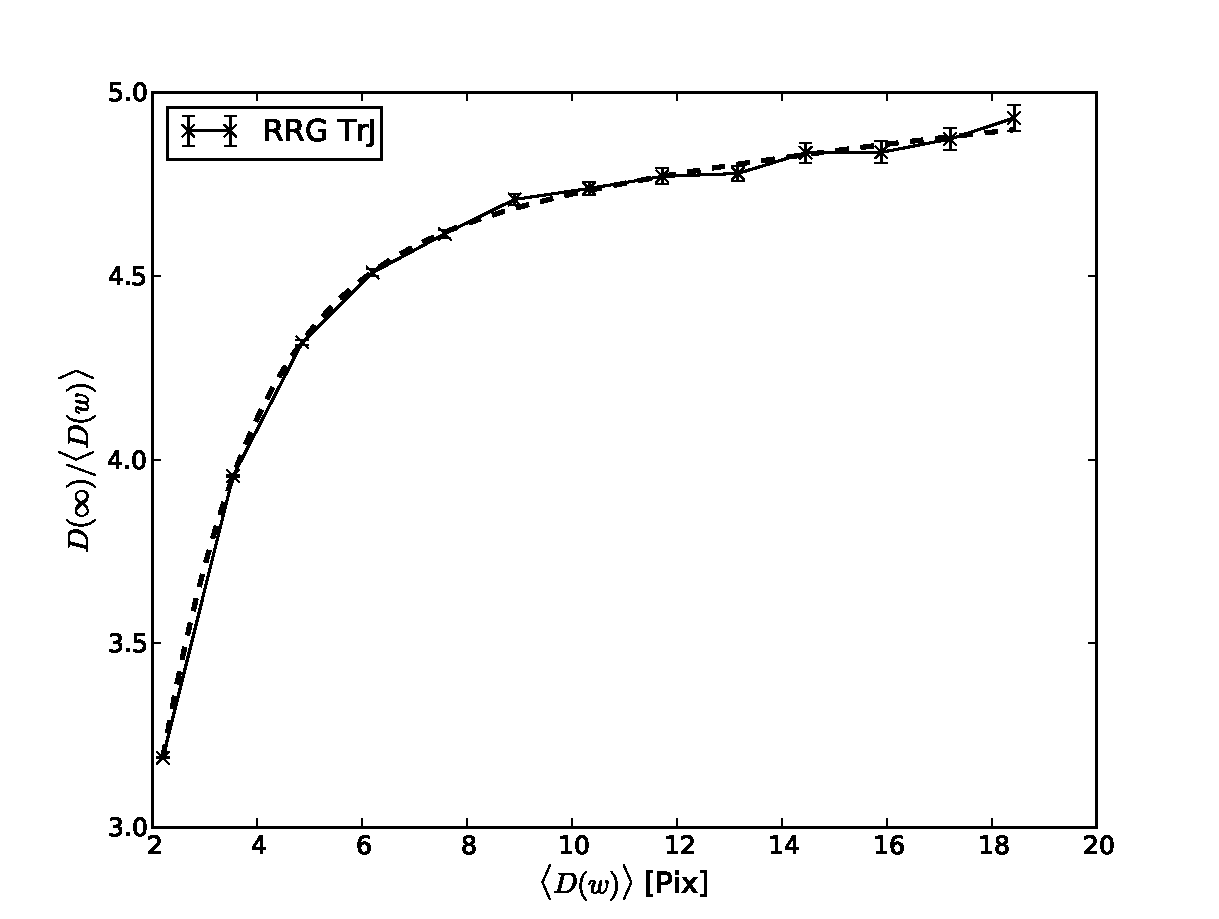
\includegraphics[width = 0.5\textwidth]{Figures/Calibration_Plots/17April2015/Size_Distributions/Calibrations/WCalib/WCalib_TrJJ_MarginalisedEllipticity.pdf}
\caption{Level-1 calibration of measured source sizes, measured from high signal--to--noise ratio image simulations, to account for the sensitivity of RRG-derived sizes to the width of the Gaussian weight function used, in this case taken to SExtractor measured flux radius}\label{Fig:WCalib}
\end{figure}

Figure \ref{Fig:SSNRCalib} shows the measured quadrupole size for a series of input Sersic scale radii for a series of measured signal--to--noise bins, where the measured signal--to--noise is taken as the ratio of SExtractor FLUX\_BEST to its equivalent error, colour coded by intrinsic surface brightness. The measured size has been corrected using the above window function calibration. On can see that for the range of scale radii considered here, the relation between the measured size and input size is linear where the signal--to--noise is large, suggesting that for high signal--to--noise sources the quadrupole size is unbiased with respect to the intrinsic size of the source. It is worth noting that even at high signal--to--noise, the respective increase in measured size due to effect of the the PSF on weight function width is not evident in these plots, suggesting that the application of the first level of calibration has successfully accounted for this trend. For low signal--to--noise sources, one can see that the quadrupole measured size does not follow the input size linearly, with a turnover seen for the largest simulated galaxies in that bin. As the measured signal--to--noise bin increases, this turnover is pushed further up and to the right, to the point where it is no longer observable on the input scales seen here. Conversely, one can see that the point of turnover trends to smaller sizes with decreasing signal--to--noise ratio. 

This turnover results from the fact that one observes only the tip of the surface brightness profile for the largest sources above the noise: for these sources are intrinsically large and faint, with a low surface brightness. As such, the wings of the surface brightness profile for an intrinsically large galaxy fall below the noise level of the image, and the observed boundary containing a given fraction of the total flux of the noisy image is smaller than the noise-free case, causing a systematic underestimation of the source's size. As a result, the relation between measured size and input size is non-monotonic, and it becomes impossible to distinguish between an intrinsically small galaxy, and an intrinsically larger body for whom only the central section of the profile is observed above poisson noise. This affects the RRG measured size in two ways: first, the SExtractor flux radius is underestimated causing a respective decrease in the width of the weight function used, and secondly beyond the point where the galaxy surface brightness profile dominates the background, any addition to the quadrupole moment is noise dominated. Since the quadrupole moment integrates beyond the measured flux radius, the down-turn is less pronounced than observed in flux radius measurement itself.

Figure \ref{Fig:SSNRCalib} therefore suggests that size measurements using quadrupole moments may not be reliable at low signal--to-noise, where the method cannot distinguish between faint, large sources and bright, small sources. At larger signal--to--noise, where the tunrover is pushed to larger instrinsic sizes, the distinction is reinforced by the reduced probability of observing a source with such a large intrinsic size. It is worth noting that \ref{Fig:SSNRCalib} suggests that in part this degeneracy can be alleviated by implementing a cut on surface brightness, thereby removing the low surface brightness sources at low signal--to--noise, however the measured surface brightness is itself affected by the same effect, complicating the effective removal of these sources from the sample.

\begin{figure*}
\centering
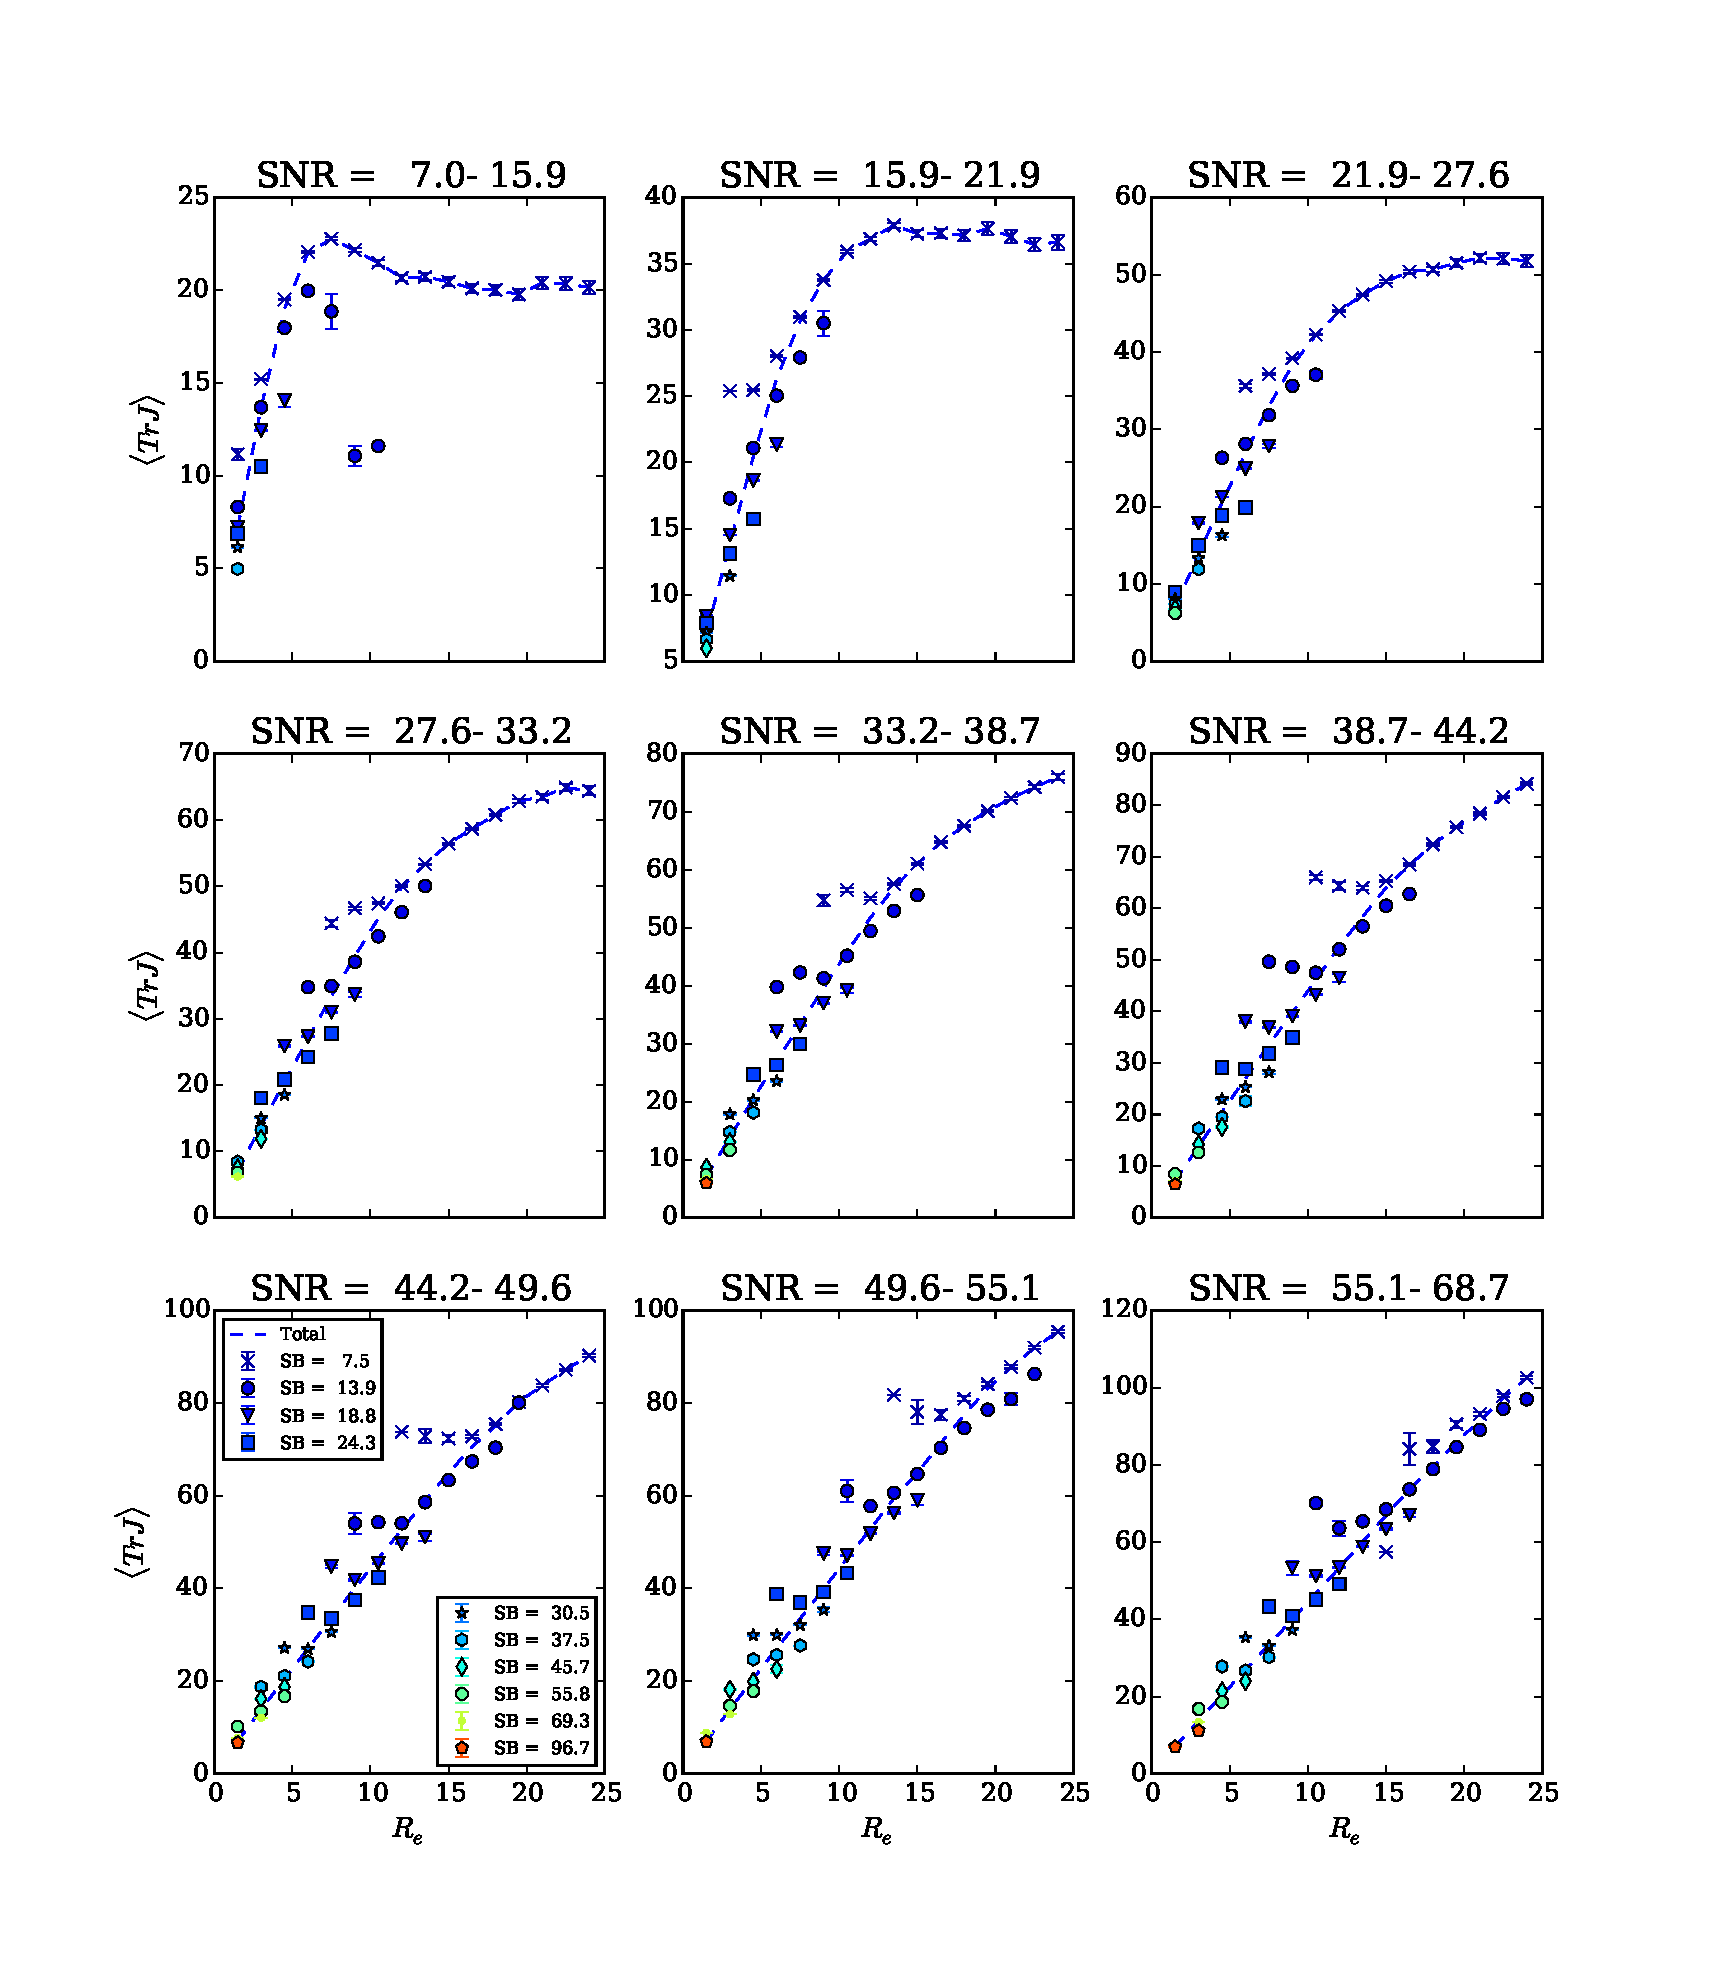
\includegraphics[width = \textwidth]{Figures/Calibration_Plots/17April2015/Size_Distributions/Calibrations/SSNR/SSNR_Calibration_ImSim_TrJ_wSB.pdf}
\caption{Plot of quadrupole measured size against input size, binned by measured signal--to--noise--ratio (SNR). Each panel corresponds to a given signal--to--noise bin, the ordinate axis gives the mean measured size using quadrupole moments for simulated Sersic galaxies with scale radius given by the co-ordinate axis. Coloured points correspond to the measurement in bins of intrinsic surface brightness, whilst the blue dashed line gives the combination of all surface brightness bins.}\label{Fig:SSNRCalib}
\end{figure*}

This investigation suggests that the use of quadrupole moments is inappropriate for accurate size measures without complicated calibration on realistic image simulations. In contrast, one may expect that the use of model-fitting methods like GALFIT my avoid most of these problems, as the model may still be fit to the peak of the surface brightness profile over the background, and thereby giving information of the profile out to the wings. Further, such a method will not require the use of a complicated weighting function which is itself a function of the measured size, and will therefore not need calibration to remove the window function (and secondary effects such as PSF and ellipticity bias), as done here.

%{\bf Figure} shows an equivalent plot, where the images have been grouped by measured surface brightness, defined as the ratio of SExtractor flux to flux radius squared. One can see that for a given measured signal--to--noise bin, the largest measured surface brightness sources correspond to the smallest intrinsic and measured sources. Similarly, for low signal--to--noise, those sources whose measured sizes are most badly biased correspond to those with smallest surface brightness as the flux under the noise level is not considered in the flux estimation. This corroborates the behaviour seen in Figure \ref{Fig:SSNRCalib}. It can be seen that those galaxies whose measured size is most seriously affected can be removed through the implementation of a surface brightness cut. Further, the use of such a cut on the sample should not be expected to introduce a bias into the analysis since surface brightness is preserved in a lensing system. As such, {\bf Figure} motivates the application for a surface brightness cut, retaining only those sources with $\mu \ge 22$. The application of such a cut removes $\sim xxxxxx$ sources.

\bsp

\label{lastpage}

\end{document}
